\documentclass{article}
\usepackage[margin=1in]{geometry}
\usepackage{amssymb}
\usepackage{authblk}

\usepackage{booktabs}
\usepackage{multirow,natbib}
\usepackage{url}
\def\bSig\mathbf{\Sigma}
\newcommand{\VS}{V\&S}
\newcommand{\tr}{\mbox{tr}}
\usepackage{amsmath,tikz}
\usetikzlibrary{calc}
\usetikzlibrary{positioning}
\title{Mixture Models for Single-Cell Assays with Application to Vaccine Studies: Supplementary Materials}
 
 \author{GREG FINAK$^{1\ast}$, 
 ANDREW MCDAVID$^{1}$,
 PRATIP CHATTOPADHYAY$^{3}$,
 MARIA DOMINGUEZ$^{3}$,
 STEVE DE ROSA$^{1,2}$,
 MARIO ROEDERER$^{3}$, 
 RAPHAEL GOTTARDO$^{1}$\\
\textit{ $^{1}$Vaccine and Infectious Disease Division, Fred Hutchinson Cancer Research Center (FHCRC), Seattle, WA\\
 $^{2}$HIV Vaccine Trials Network, Fred Hutchinson Cancer Research Center (FHCRC), Seattle, WA\\
 $^{3}$Vaccine Research Center, NIAID, NIH, 40 Convent Drive, Rm 5509, Bethesda, MD 20892}}
\date{}
\begin{document}
\maketitle
\appendix
%\renewcommand{\thesection}{\Alph{section}}
\renewcommand{\thesubsection}{Appendix \Alph{subsection}:}
%\setcounter{section}{1}
\setcounter{subsection}{0}
%\setcounter{figure}{0}
\renewcommand{\figurename}{\textbf{Supplementary Figure}}
\renewcommand{\thefigure}{\textbf{\arabic{figure}}}
\setcounter{figure}{0}
%\todo[inline]{Note that the Supplementary Information section needs corrections to notation and overall}

\section*{}

\subsection{Constrained beta-binomial model}
\label{supp:constrained}
We can define a model where we constrain the stimulated proportions under the alternative model such that $p^{(s)}>p^{(u)}$. In this case, the only changes required are for the alternative marginal likelihood $\mathrm{L}_1$ defined in the main manuscript by (1). Due to the constraint, the normalizing constant of the prior under the alternative (model ${\cal M}_1$) is not given by $\mathrm{B}(\alpha^{(u)},\beta^{(u)})\mathrm{B}(\alpha^{(s)},\beta^{(s)})$ but requires computing \[
Z(\alpha^{(u)}, \beta^{(u)}, \alpha^{(s)}, \beta^{(s)})=\int_{0}^1{p^{(u)}}^{\alpha^{(u)}-1}(1-p^{(u)})^{\beta^{(u)}-1}\int_{p^{(u)}}^1 p^{(s)\alpha^{(s)}-1}(1-p^{(s)})^{\beta^{(s)}-1}dp^{(s)}dp^{(u)}.
\]
Using this expression, the constrained alternative marginal likelihood can be written as
\[
\mathrm{L}_1(\alpha^{(u)},\beta^{(u)},\alpha^{(s)},\beta^{(s)}|\mathbf{y}_i)
=\binom{N^{(u)}_{i}}{n^{(u)}_{i}} \binom{N^{(s)}_{i}}{n^{(s)}_{i}}\frac{Z(n^{(u)}_{i}+\alpha^{(u)},N^{(u)}_{i}-n^{(u)}_{i}+\beta^{(u)},n^{(s)}_{i}+\alpha^{(s)},N^{(s)}_{i}-n^{(s)}_{i}+\beta^{(s)})}{Z(\alpha^{(u)},\beta^{(u)},\alpha^{(s)},\beta^{(s)})}.
\label{model2:constrained}
\]
In general, there is no closed-form expression for $Z(\cdot)$, and a numerical approximation must be used. Let us denote by $\tilde{Z}(\alpha^{(u)}, \beta^{(u)}, \alpha^{(s)}, \beta^{(s)})$ the approximation. A natural way to estimate $\tilde{Z}$ is to use Monte Carlo integration. Indeed, we can write
\begin{equation}
\tilde{Z}(\alpha^{(u)}, \beta^{(u)}, \alpha^{(s)}, \beta^{(s)})=\mathrm{B}(\alpha^{(u)},\beta^{(u)})\mathrm{B}(\alpha^{(s)},\beta^{(s)})\int_{0}^1\frac{{p^{(u)}}^{\alpha^{(u)}-1}(1-p^{(u)})^{\beta^{(u)}-1}}{\mathrm{B}(\alpha^{(u)},\beta^{(u)})}[1-F_{\alpha^{(s)},\beta^{(s)}}(p^{(u)})]dp^{(u)}
\label{equ:normZ}
\end{equation}
where $F_{\alpha^{(s)},\beta^{(s)}}$ is the cumulative distribution function of a beta random variable with parameters $\alpha^{(s)}$ and $\beta^{(s)}$. Using this identity, it can be seen that $\tilde{Z}(\alpha^{(u)}, \beta^{(u)}, \alpha^{(s)}, \beta^{(s)})$ can be approximated by
\[
\tilde{Z}(\alpha^{(u)}, \beta^{(u)}, \alpha^{(s)}, \beta^{(s)})\approx\mathrm{B}(\alpha^{(u)},\beta^{(u)})\mathrm{B}(\alpha^{(s)},\beta^{(s)})\sum_{k=1}^K[1-F_{\alpha^{(s)},\beta^{(s)}}(X_k)]
\]
where the $X_k$'s are \textit{iid} beta distributed random variables with parameters $\alpha^{(s)}$, $\beta^{(s)}$ and $K$ is the number of terms used in the Monte Carlo approximation. This approximation works relatively well with our EM implementation and does not significantly increase the computing time.
Unfortunately, the number of terms (\textit{i.e.} value of $K$) required for the approximation to be good might be large and computing such a normalizing constant at each iteration would significantly slow down our MCMC implementation. As it tuns out, a better approximation
can be obtained when $\alpha^{(s)}$ and $\beta^{(s)}$ are integers. In this case, the cdf function in \eqref{equ:normZ} can be calculated exactly using integration by parts, as follows,
\[
F_{\alpha^{(s)},\beta^{(s)}}(p^{(u)})=\sum_{j=\beta^{(s)}}^{\beta^{(s)}+\alpha^{(s)}-1} \frac{(\beta^{(s)}+\alpha^{(s)}-1)!}{j!(\beta^{(s)}+\alpha^{(s)}-j)!}(1-p^{(u)})^jp^{(u)\beta^{(s)}+\alpha^{(s)}-j}.
\label{eq:IBident}
\]
Then using this identity, we obtain
\begin{align*}
Z(\alpha^{(u)}, \beta^{(u)}, \alpha^{(s)}, \beta^{(s)})&=\mathrm{B}(\alpha^{(s)},\beta^{(s)})\sum_{j=\beta^{(s)}}^{\beta^{(s)}+\alpha^{(s)}-1}\frac{(\beta^{(s)}+\alpha^{(s)}-1)!}{j!(\beta^{(s)}+\alpha^{(s)}-j)!}\int_{0}^1(1-p^{(u)})^{\beta^{(u)}-1+j}p^{(u)\alpha^{(u)}-1+\beta^{(s)}+\alpha^{(s)}-j}dp^{(u)}\\
&=\mathrm{B}(\alpha^{(s)},\beta^{(s)})\sum_{j=\beta}^{(s)\beta^{(s)}+\alpha^{(s)}-1}\frac{(\beta^{(s)}+\alpha^{(s)}-1)!}{j!(\beta^{(s)}+\alpha^{(s)}-j)!}\mathrm{B}(\beta^{(u)}+j)\mathrm{B}(\alpha^{(u)}+\beta^{(s)}+\alpha^{(s)}-j).
\label{equ:normZ}
\end{align*}
Typically, in ICS data $\alpha^{(u)}$ is relatively small leading to relatively few terms in the sum. However, the use of this exact identity in our MCMC algorithm requires the use of discrete priors on $\alpha^{(s)}$ and $\beta^{(s)}$, which can be restrictive in terms of fit (\textit{e.g.},  if the true $\alpha^{(s)}$ is less than one) and can render mixing in the MCMC more difficult. In addition, even though the computation is exact and much faster for small values of $\alpha^{(s)}$, which is typically the case with ICS data, it is still more demanding than the unconstrained model. In our case, we have decided to use the unconstrained model and simply fix the $z_i$ to zero if the empirical proportion for the un-stimulated sample, $p^{(u)}$, is greater than that of the stimulation sample, $p^{(s)}$. Indeed, in the one-sided case, if $p^{(u)}>p^{(s)}$ the associated individual should be a non-responder and thus $z_i=0$. In our experience, this computational shortcut performs just as well as the true one-sided implementation while being computationally much less demanding.

\subsection{Computational details for the beta-binomial model}
\noindent\textbf{Marginal likelihood derivations}\\
For a given subject $i$, the null marginal likelihood is obtained after integrating out the prior from the likelihood for model ${\cal M}_0$, as follows,
\[
\begin{split}
\mathrm{L_0}(\alpha^{(u)},\beta^{(u)}|n^{(s)}_{i},n^{(u)}_{i}) =&\int_0^1 \mathrm{Pr}(n^{(s)}_{i},n^{(u)}_{i}|p^{(u)})\pi(p^{(u)}|\alpha^{(u)},\beta^{(u)})\mathrm{d}p^{(u)}\\
=& \int_0^1Pr(n^{(s)}|p^{(u)})Pr(n^{(u)}|p^{(u)})\pi(p^{(u)}|\alpha^{(u)},\beta^{(u)}) \mathrm{d}p^{(u)}\\
=&\int_0^1\binom{N^{(s)}}{n^{(s)}}p^{(s)n^{(s)}}(1-p^{(u)})^{N^{(s)}-n^{(s)}}\binom{N^{(u)}}{n^{(u)}}p^{(u)n^{(u)}}(1-p^{(u)})^{N^{(u)}-n^{(u)}}\cdot \\&\frac{1}{\mathrm{B}(\alpha^{(u)},\beta^{(u)})}p^{(u)\alpha^{(u)}-1}(1-p^{(u)})^{\beta^{(u)}-1} \mathrm{d}p^{(u)}\\
=&\binom{N^{(s)}}{n^{(s)}}\binom{N^{(u)}}{n^{(u)}}\frac{1}{\mathrm{B}(\alpha^{(u)},\beta^{(u)})}\int_0^1 p^{(u)n^{(s)}+n^{(u)}+\alpha^{(u)}-1}(1-p^{(u)})^{N^{(s)}+N^{(u)}-n^{(s)}-n^{(u)}+\beta^{(u)}-1} \mathrm{d}p^{(u)}\\
=&\binom{N^{(s)}}{n^{(s)}}\binom{N^{(u)}}{n^{(u)}}\frac{\mathrm{B}(n^{(s)}+n^{(u)}+\alpha^{(u)},N^{(s)}+N^{(u)}-n^{(s)}-n^{(u)}+\beta^{(u)})}{\mathrm{B}(\alpha^{(u)},\beta^{(u)})}.
\end{split}
\]


\noindent Similarly, the alternative marginal likelihood for a given subject is defined as,
\[
\begin{split}
\mathrm{L_1}(\alpha^{(u)},\beta^{(u)},\alpha^{(s)},\beta^{(s)}|n^{(s)}_{i},n^{(u)}_{i}) =&\int_0^1\int_0^1 \mathrm{Pr}(n^{(s)}_{i},n^{(u)}_{i}|p^{(u)},p^{(s)})\pi(p^{(u)},p^{(s)}|\alpha^{(u)},\beta^{(u)},\alpha^{(s)},\beta^{(s)})\mathrm{d}p^{(s)}\mathrm{d}p^{(u)} \\
=&\int_0^1\int_0^1\binom{N^{(s)}}{n^{(s)}}p^{(s)n^{(s)}}(1-p^{(s)})^{N^{(s)}-n^{(s)}}\binom{N^{(u)}}{n^{(u)}}p^{(u)n^{(u)}}(1-p^{(u)})^{N^{(u)}-n^{(u)}} \cdot\\  &\frac{1}{\mathrm{B}(\alpha^{(u)},\beta^{(u)})}p^{(u)\alpha^{(u)}-1}(1-p^{(u)})^{\beta^{(u)}-1}
\frac{1}{\mathrm{B}(\alpha^{(s)},\beta^{(s)})}p^{(s)\alpha^{(s)}-1}(1-p^{(s)})^{\beta^{(s)}-1} \mathrm{d}p^{(s)}\mathrm{d}p^{(u)}\\
=&\binom{N^{(s)}}{n^{(s)}}\binom{N^{(u)}}{n^{(u)}}\frac{1}{\mathrm{B}(\alpha^{(u)},\beta^{(u)})}\frac{1}{\mathrm{B}(\alpha^{(s)},\beta^{(s)})}\int_0^1 p^{(u)n^{(u)}+\alpha^{(u)}-1}(1-p^{(u)})^{N^{(u)}-n^{(u)}+\beta^{(u)}-1} \cdot\\
&\int_0^1 p^{(s)n^{(s)}+\alpha^{(s)}-1}(1-p^{(s)})^{N^{(s)}-n^{(s)}+\beta^{(s)}-1}\mathrm{d}p^{(s)}\mathrm{d}p^{(u)} \\
=&\binom{N^{(s)}}{n^{(s)}}\binom{N^{(u)}}{n^{(u)}}\frac{\mathrm{B}(n^{(u)}+\alpha^{(u)},N^{(u)}-n^{(u)}+\beta^{(u)})\mathrm{B}(n^{(s)}+\alpha^{(s)},N^{(s)}-n^{(s)}+\beta^{(s)})}{\mathrm{B}(\alpha^{(u)},\beta^{(u)})\mathrm{B}(\alpha^{(s)},\beta^{(s)})}.
\end{split}
\]
%and taking the product over subjects leads to
%\[
%\mathrm{L_1}(\alpha_u,\beta_u,\alpha_s,\beta_s|\mathbf{n}_{s},\mathbf{n}_{u}) = \prod_{i=1}^P \binom{N_{si}}{n_{si}}\binom{N_{ui}}{n_{ui}}\frac{\mathrm{B}(n_{ui}+\alpha_u,N_{ui}-n_{ui}+\beta_u)\mathrm{B}(n_{si}+\alpha_s,N_{si}-n_{si}+\beta_s)}{\mathrm{B}(\alpha_u,\beta_u)\mathrm{B}(\alpha_s,\beta_s)}
%\]

\noindent\textbf{MCMC algorithm}\\
In what follows, we use $(x|y)$ to denote the conditional distribution of $x$ given $y$. In particular, we use $(x|\cdots)$ to denote the distribution of $x$ conditional on everything else in the model. Our MCMC algorithms cycles through the following steps:
\begin{enumerate}
\item Update each $\alpha^{(u)}, \beta^{(u)}, \alpha^{(s)}$ and $\beta^{(s)}$ by Metropolis-Hastings using a Gaussian symmetric proposal where the variance of the proposal is tuned for each parameter using the approach of~\cite{Gelman:2004tc}.
\item Update $w$ by Gibbs sampling using the full conditional,
\[
(w|\cdots)\sim \mathrm{Beta}(\sum_i z_i,\sum_i (1-z_i)).
\]
\item for each $i$, update $z_i$ by Gibbs sampling using the following full conditional,
\[
(z_i|\cdots)\sim\mathrm{B}(1,p_i).
\]
where,
\[
p_i=\frac{w\cdot\mathrm{L_1}(\alpha^{(u)},\beta^{(u)},\alpha^{(s)},\beta^{(s)}| n^{(u)}_{i},n^{(s)}_{i})}{w\cdot\mathrm{L_1}(\alpha^{(u)},\beta^{(u)},\alpha^{(s)},\beta^{(s)}|n^{(u)}_{i},n^{(s)}_{i})+(1-w)\cdot\mathrm{L_0}(\alpha^{(u)},\beta^{(u)}|n^{(u)}_{i},n^{(s)}_{i})}.
\]
\end{enumerate}
For each updated parameter, step 1 above involves the calculation of the following acceptance ratio, (e.g. $\alpha^{(u)}$, below),
\[
\begin{split}
\frac{\mathrm{L}(\alpha^{(u)\text{new}},\beta^{(u)},\alpha^{(s)},\beta^{(s)}|\cdots)\pi(\alpha^{(u)\text{new}})}{\mathrm{L}(\alpha^{(u)},\beta^{(u)},\alpha^{(s)},\beta^{(s)}|\cdots)\pi(\alpha^{(u)})}\\
\end{split}
\]
where $L$ is the complete marginal likelihood conditional on $\mathbf{z}$ defined as,
\[
\mathrm{L}(\alpha^{(u)},\beta^{(u)},\alpha^{(s)},\beta^{(s)}|\mathbf{n}^{(u)},\mathbf{n}^{(s)},\mathbf{z})=\prod_i\mathrm{L}_{z_i}(\alpha^{(u)},\beta^{(u)},\alpha^{(s)},\beta^{(s)}|\mathbf{n}^{(u)},\mathbf{n}^{(s)})
\]
and $\pi$ is the prior distribution of $\alpha^{(u)}$. The obvious changes in the above expression are made for the acceptance ratios of $\alpha^{(s)},\beta^{(s)},\beta^{(u)}$. In our case each parameter has the same exponential prior with mean $1,000$

\subsection{Computational details for the Dirichlet-multinomial model}
\noindent\textbf{Marginal likelihood derivations}\\
Because our Dirichlet-multinomial is a direct extension of the beta-binomial model, the marginal likelihoods are obtained in the exact same fashion.
For a given subject, the null marginal likelihood is defined as
\[
\begin{split}
\mathrm{L_0}(\boldsymbol{\alpha}^{(u)}|\mathbf{n}^{(s)}_{i},\mathbf{n}^{(u)}_{i})=&\idotsint\mathrm{Pr}(\mathbf{n}^{(s)}_{i},\mathbf{n}^{(u)}_{i}|\mathbf{p}^{(u)})\pi(\mathbf{p}^{(u)}|\boldsymbol{\alpha}^{(u)})\mathrm{d}\mathbf{p}^{(u)}\\
=&\idotsint \frac{\mathbf{N}^{(s)}!}{\prod_k {n}^{(s)}_{ik}!}\prod_k p^{(u)n^{(s)}_{ik}}_{k} \frac{\mathbf{N}^{(u)}!}{\prod_k {n}^{(u)}_{ik}!}\prod_k p^{(u)n^{(u)}_{ik}}_{k}\frac{1}{\mathrm{B}(\boldsymbol{\alpha}^{(u)})}\prod_k p^{(u)\alpha^{(u)}_{k}-1}_{k}\mathrm{d}\mathbf{p}^{(u)}\\
=&\frac{\mathbf{N}^{(s)}!}{\prod_k {n}^{(s)}_{ik}!}\frac{\mathbf{N}^{(u)}!}{\prod_k {n}^{(u)}_{ik}!}\frac{1}{\mathrm{B}(\boldsymbol{\alpha}^{(u)})}\int_0^1 \prod_k p^{(u)n^{(s)}_{ik}+n^{(u)}_{ik}+\alpha^{(u)}_{k}-1}_{k}\mathrm{d}\mathbf{p}^{(u)}\\
=&\frac{\mathbf{N}^{(s)}!}{\prod_k {n}^{(s)}_{ik}!}\frac{\mathbf{N}^{(u)}!}{\prod_k {n}^{(u)}_{ik}!}\frac{\mathrm{B}(\mathbf{n}^{(s)}_{i}+\mathbf{n}^{(u)}+\boldsymbol{\alpha}^{(u)})}{\mathrm{B}(\boldsymbol{\alpha}^{(u)})}
\end{split}
\]
%The product over all $P$ observations gives the marginal likelihood,
%\[
%\mathrm{L_0}(\boldsymbol{\alpha}_u|\mathbf{n}_s,\mathbf{n}_u)=\prod_{i=0}^P \frac{\mathbf{N}_{si}!}{\prod_k \mathbf{n}_{sik}!}\frac{\mathbf{N}_{ui}!}{\prod_k \mathbf{n}_{uik}!}\frac{\mathrm{B}(\mathbf{n}_{si}+\mathbf{n}_{ui}+\boldsymbol{\alpha}_{u})}{\mathrm{B}(\boldsymbol{\alpha}_{u})}
%\]

\noindent Similarly, the alternative marginal likelihood for a given subject is:
\[
\begin{split}
\mathrm{L_1}(\boldsymbol{\alpha}^{(u)},\boldsymbol{\alpha}^{(s)}|\mathbf{n}^{(u)}_{i},\mathbf{n}^{(s)}_{i})
%=&\int_0^1\int_0^1 \mathcal{M}(\mathbf{N}_u,\mathbf{p}_u)\mathcal{M}(\mathbf{N}_s,\mathbf{p}_s)\mathrm{Dir}(\boldsymbol{\alpha}_u)\mathrm{Dir}(\boldsymbol{\alpha}_s)\mathrm{d}\mathbf{p}_u\mathrm{d}\mathbf{p}_s\\
=&\frac{\mathbf{N}^{(s)}!}{\prod_k {n}^{(s)}_{ik}!}\frac{\mathbf{N}^{(u)}!}{\prod_k {n}^{(u)}_{ik}!}\frac{1}{\mathrm{B}(\boldsymbol{\alpha}^{(u)})\mathrm{B}(\boldsymbol{\alpha}^{(s)})}\idotsint\prod_k p^{(u)n^{(u)}_{ik}+\alpha^{(u)}_{k}-1}_{k}\idotsint \prod_k p^{(s)n^{(s)}_{ik}+\alpha^{(s)}_{k}-1}_{k}\mathrm{d}\mathbf{p}^{(u)}\mathrm{d}\mathbf{p}^{(s)}\\
=&\frac{\mathbf{N}^{(s)}!}{\prod_k {n}^{(s)}_{ik}!}\frac{\mathbf{N}^{(u)}!}{\prod_k {n}^{(u)}_{ik}!}\frac{\mathrm{B}(\mathbf{n}^{(u)}_{i}+\boldsymbol{\alpha}^{(u)})\mathrm{B}(\mathbf{n}^{(s)}_{i}+\boldsymbol{\alpha}^{(s)})}{\mathrm{B}(\boldsymbol{\alpha}^{(u)})\mathrm{B}(\boldsymbol{\alpha}^{(s)})}.
\end{split}
\]
\noindent\textbf{MCMC algorithm}\\
The MCMC algorithm for the Dirichlet-multinomial model is analogous to the beta-binomial, above. The parameter vectors $\boldsymbol{\alpha}^{(s)},\boldsymbol{\alpha}^{(u)}$ are updated component-wise:
\begin{enumerate}
\item  Update each $\alpha^{(s)}_{k}$, $\alpha^{(u)}_{k}$ using a Gaussian symmetric proposal distribution with the variance of each proposal tuned using the approach of~\cite{Gelman:2004tc}.
\item Update $w$ by Gibbs sampling using the full conditional,
\[
(w|\cdots)\sim\mathrm{Beta}(\sum_i z_i,\sum_i(1-z_i))
\]
\item For each $i$, update $z_i$ using the full conditional,
\[
(z_i|\cdots)\sim \mathrm{B}(1,p_i)
\]
where
\[
p_i = \frac{w\cdot\mathrm{L_1}(\boldsymbol{\alpha}^{(u)},\boldsymbol{\alpha}^{(s)}|\mathbf{n}^{(s)}_{i},\mathbf{n}^{(u)}_{i})}{w\cdot\mathrm{L_1}(\boldsymbol{\alpha}^{(u)},\boldsymbol{\alpha}^{(s)}|\mathbf{n}^{(s)}_{i},\mathbf{n}^{(u)}_{i})+(1-w)\cdot\mathrm{L_0}(\boldsymbol{\alpha}^{(u)}|\mathbf{n}^{(s)}_{i},\mathbf{n}^{(u)}_{i})}
\]
For each parameter component updated in step 1 above, compute the acceptance ratio (e.g. $\alpha^{(u)}_{k}$, below):
\[
\frac{\mathrm{L}(\alpha^{(u)\text{new}}_{k},\boldsymbol{\alpha}^{(u)}_{\{-k\}},\boldsymbol{\alpha}^{(s)}|\cdots)\pi(\alpha^{(u)\text{new}}_{k})}{\mathrm{L}(\boldsymbol{\alpha}^{(u)},\boldsymbol{\alpha}^{(s)}|\cdots)\pi(\alpha^{(u)}_{k})}\\
\]

where $\pi$ is the prior distribution of the parameter, and $\boldsymbol{\alpha}^{(u)}_{\{-k\}} = \{\alpha^{(u)}_{j} :  j\neq k\}$. Again, we have used the same exponential prior with mean 1,000 for each parameter. $\mathrm{L}$ is the complete marginal likelihood conditional on $\mathbf{z}$, defined as
\[
\mathrm{L}(\boldsymbol{\alpha}^{(u)},\boldsymbol{\alpha}^{(s)}|\mathbf{n}^{(s)}_{i},\mathbf{n}^{(u)}_{i},\mathbf{z}) = \prod_i \mathrm{L}_{z_i}(\boldsymbol{\alpha}^{(u)},\boldsymbol{\alpha}^{(s)}|\mathbf{n}^{(s)}_{i},\mathbf{n}^{(u)}_{i}).
\]

\end{enumerate}

\begin{figure} %  figure placement: here, top, bottom, or page
   \centering
%   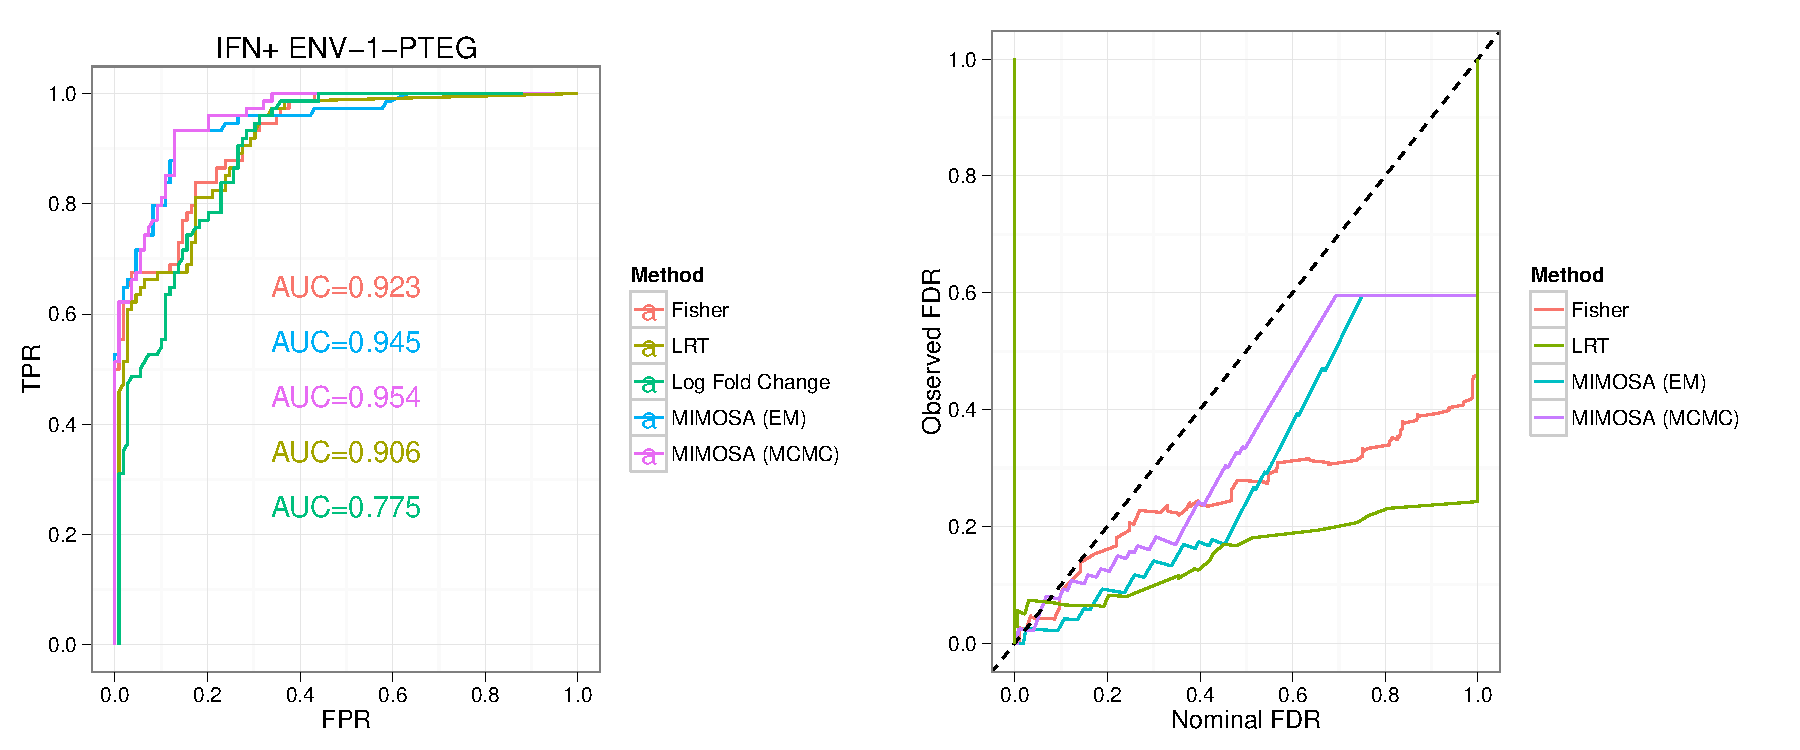
\includegraphics[width=.75\columnwidth]{Figures/2}\\
%   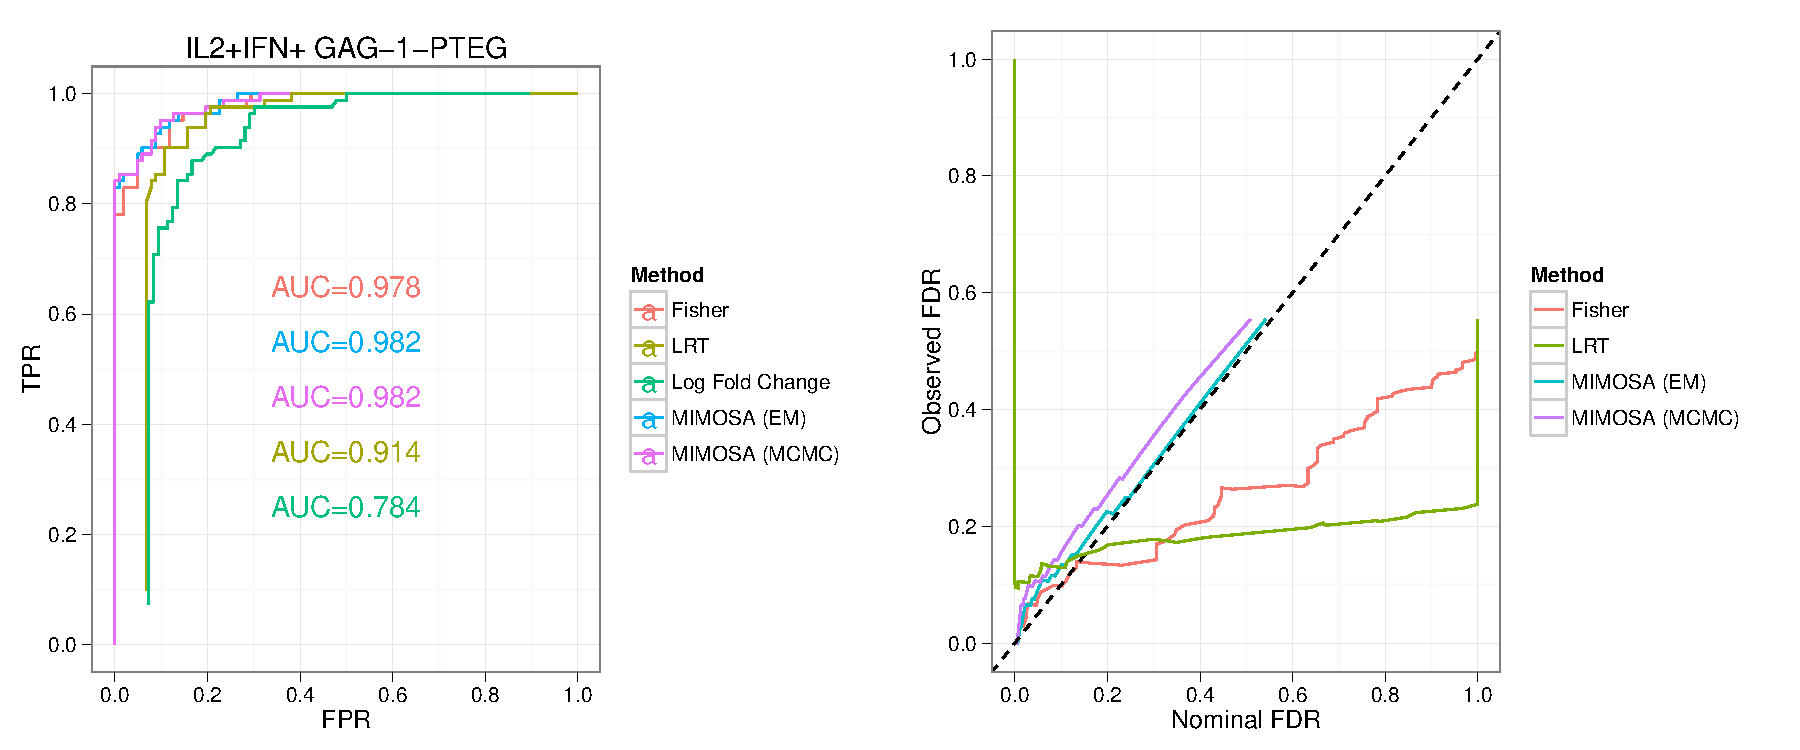
\includegraphics[width=.75\columnwidth]{Figures/12}
\begin{tikzpicture} [auto, node distance=0cm]
 \node at (0,) (A) {
 \begin{tikzpicture}
    \node[anchor=south west, inner sep=0] at (0,0) (b) {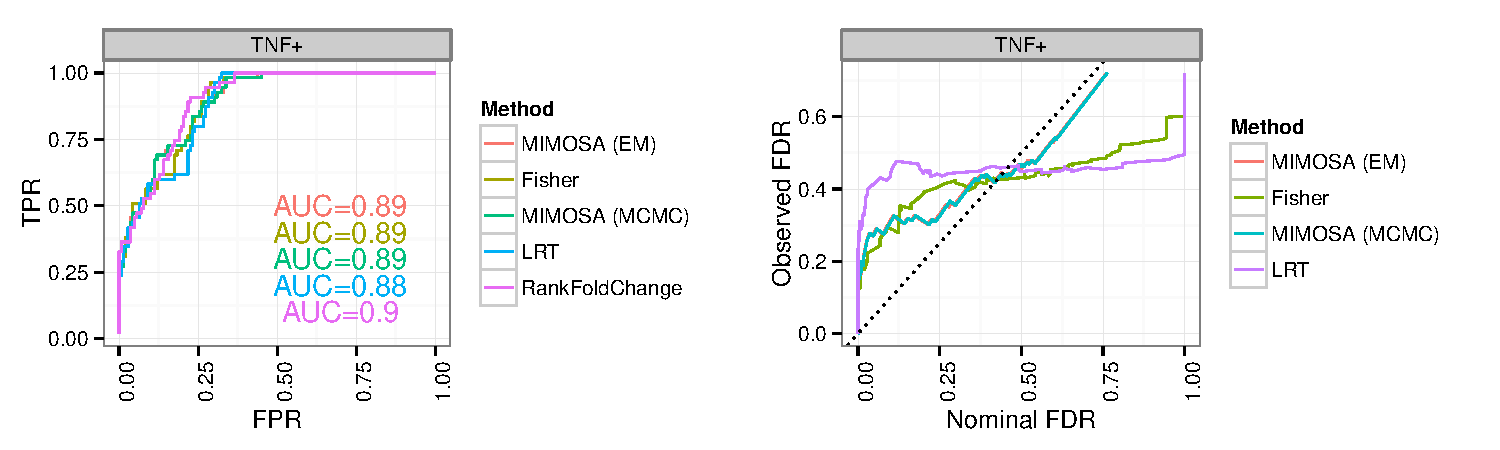
\includegraphics[width=.5\columnwidth]{Figures/revised_3.pdf}};
        \begin{scope}[x={(b.south east)},y={(b.north west)}]
        \node at (0,1) [font=\tiny\sffamily] {A} ;
                \end{scope}
        \end{tikzpicture}
 };
 \node [right=of A] (B) {
 \begin{tikzpicture}
    \node[anchor=south west, inner sep=0] at (0,0) (c) {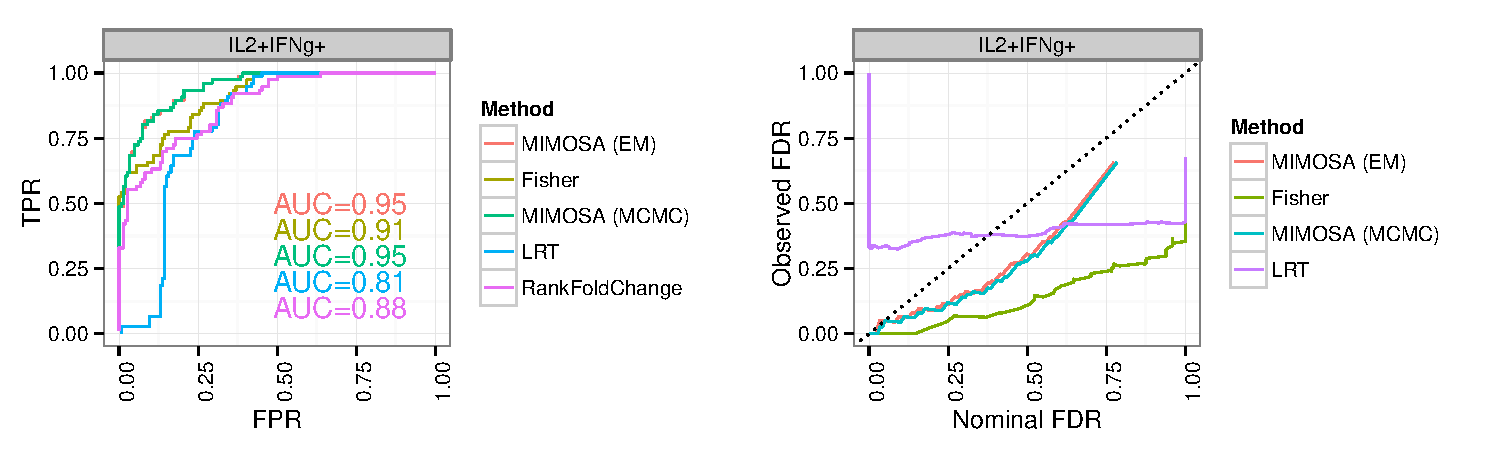
\includegraphics[width=.5\columnwidth]{Figures/revised_5.pdf}};
        \begin{scope}[x={(c.south east)},y={(c.north west)}]
        \node at (0,1) [font=\tiny\sffamily] {B} ;
        \end{scope}
        \end{tikzpicture}
};
\node [below=of A] (C) {
\begin{tikzpicture}
    \node[anchor=south west, inner sep=0] at (0,0) (d) {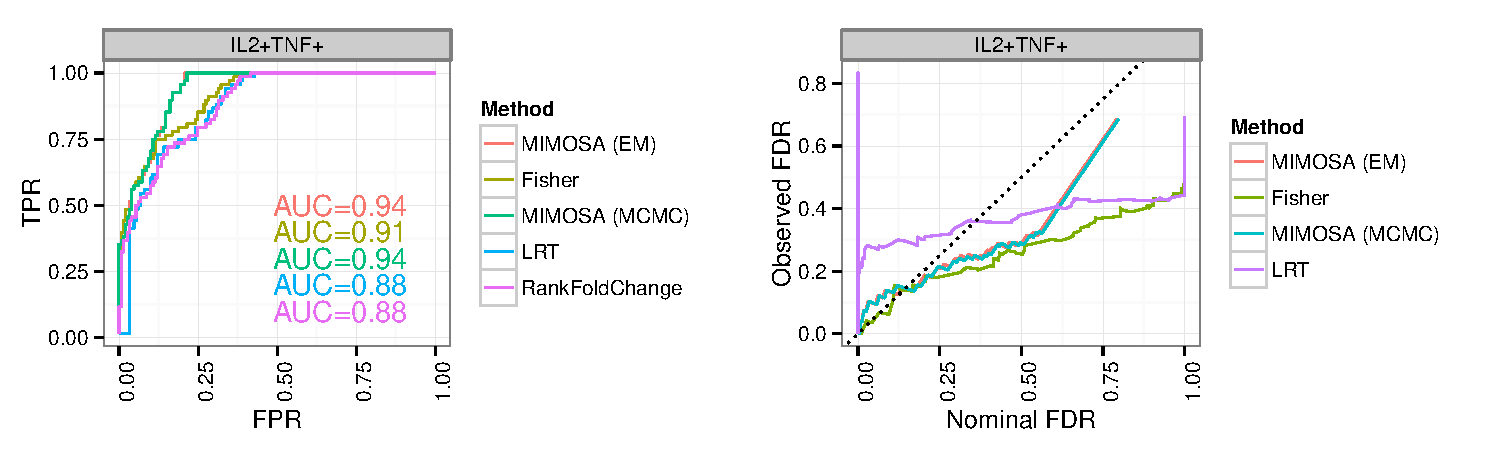
\includegraphics[width=.5\columnwidth]{Figures/revised_6.pdf}};
        \begin{scope}[x={(d.south east)},y={(d.north west)}]
        \node at (0,1) [font=\tiny\sffamily] {C} ;
                \end{scope}
        \end{tikzpicture}
};
\node [right=of C] (D) {
\begin{tikzpicture}
    \node[anchor=south west, inner sep=0] at (0,0) (e) {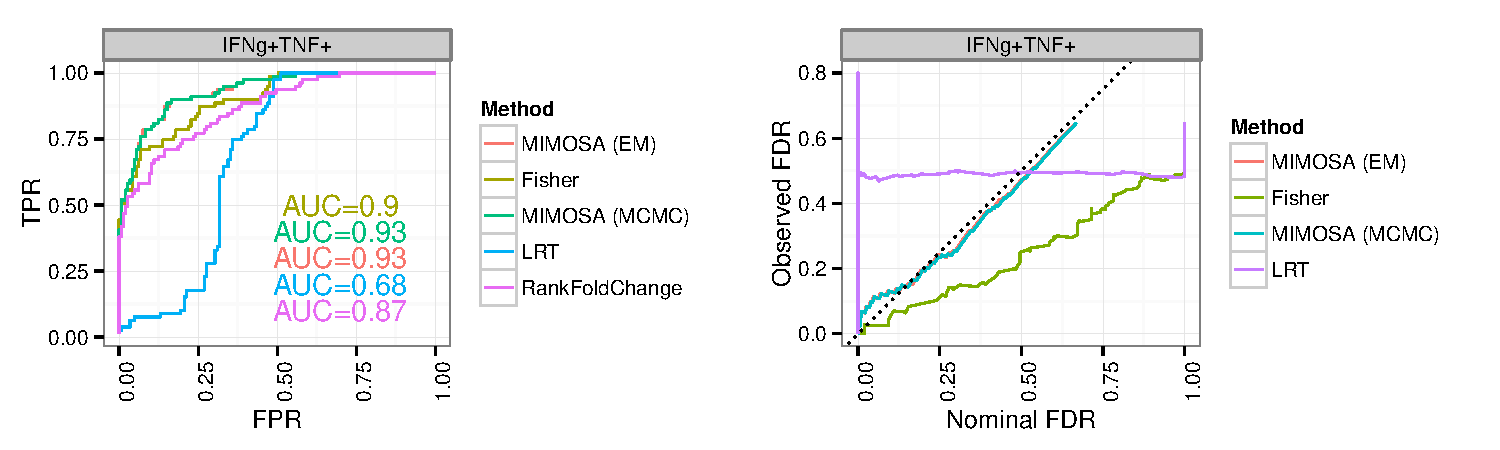
\includegraphics[width=.5\columnwidth]{Figures/revised_7.pdf}};
        \begin{scope}[x={(d.south east)},y={(d.north west)}]
        \node at (0,1) [font=\tiny\sffamily] {D} ;
                \end{scope}
        \end{tikzpicture}
 };
 \node [below=of C] (E) {
\begin{tikzpicture}
    \node[anchor=south west, inner sep=0] at (0,0) (e) {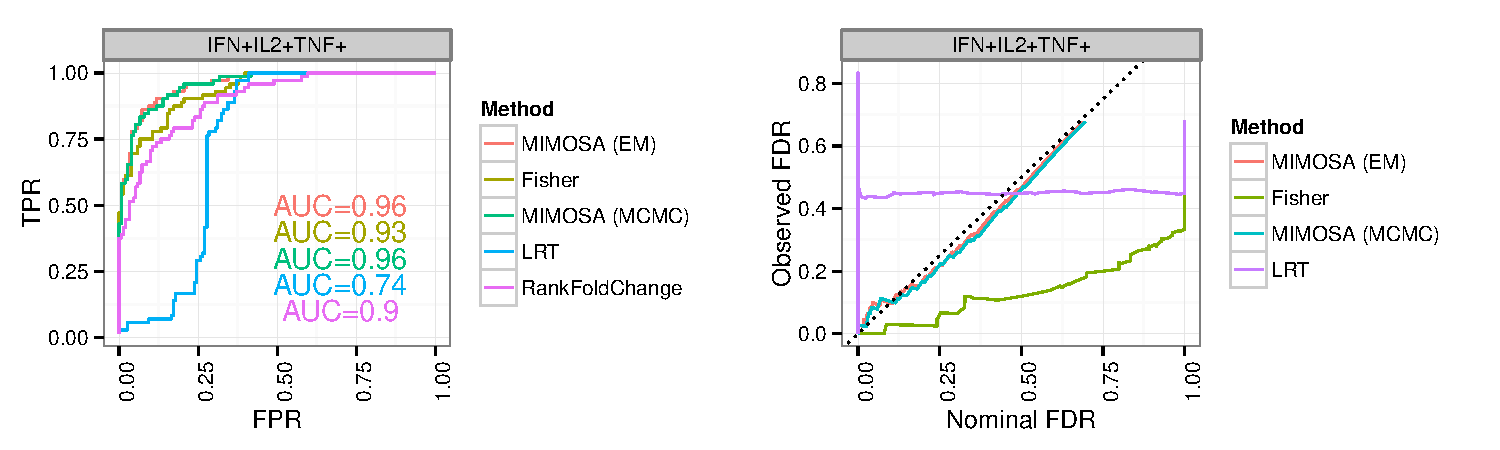
\includegraphics[width=.5\columnwidth]{Figures/revised_8.pdf}};
        \begin{scope}[x={(d.south east)},y={(d.north west)}]
        \node at (0,1) [font=\tiny\sffamily] {E} ;
                \end{scope}
        \end{tikzpicture}
 };
   % \node[anchor=south west, inner sep=0] at (8,-7.5){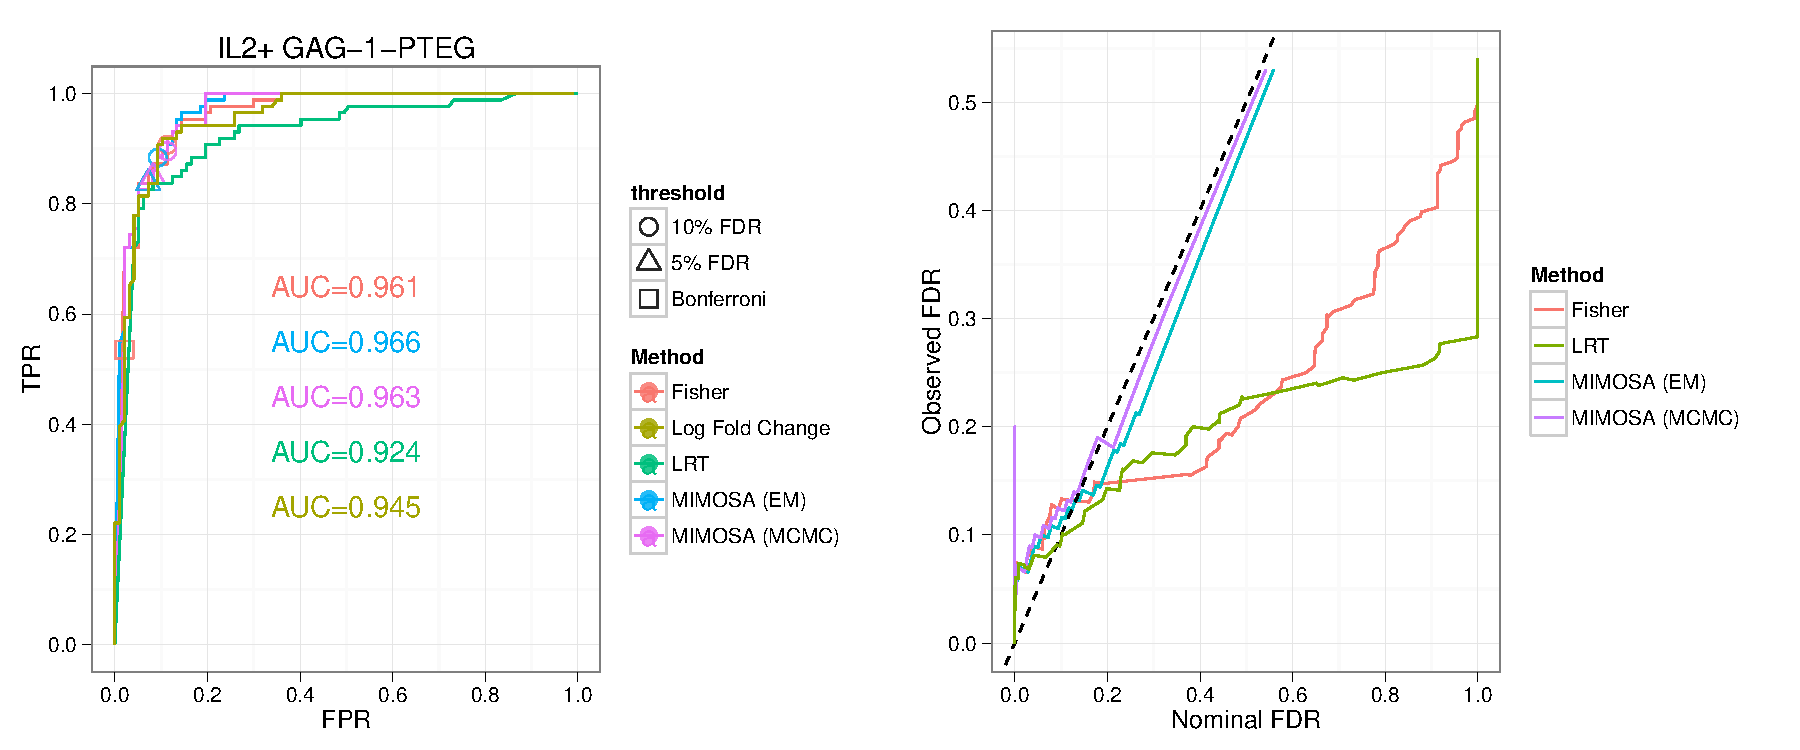
\includegraphics[width=.5\columnwidth]{Figures/8}};
   % \node[anchor=south west, inner sep=0] at (0,-11.25){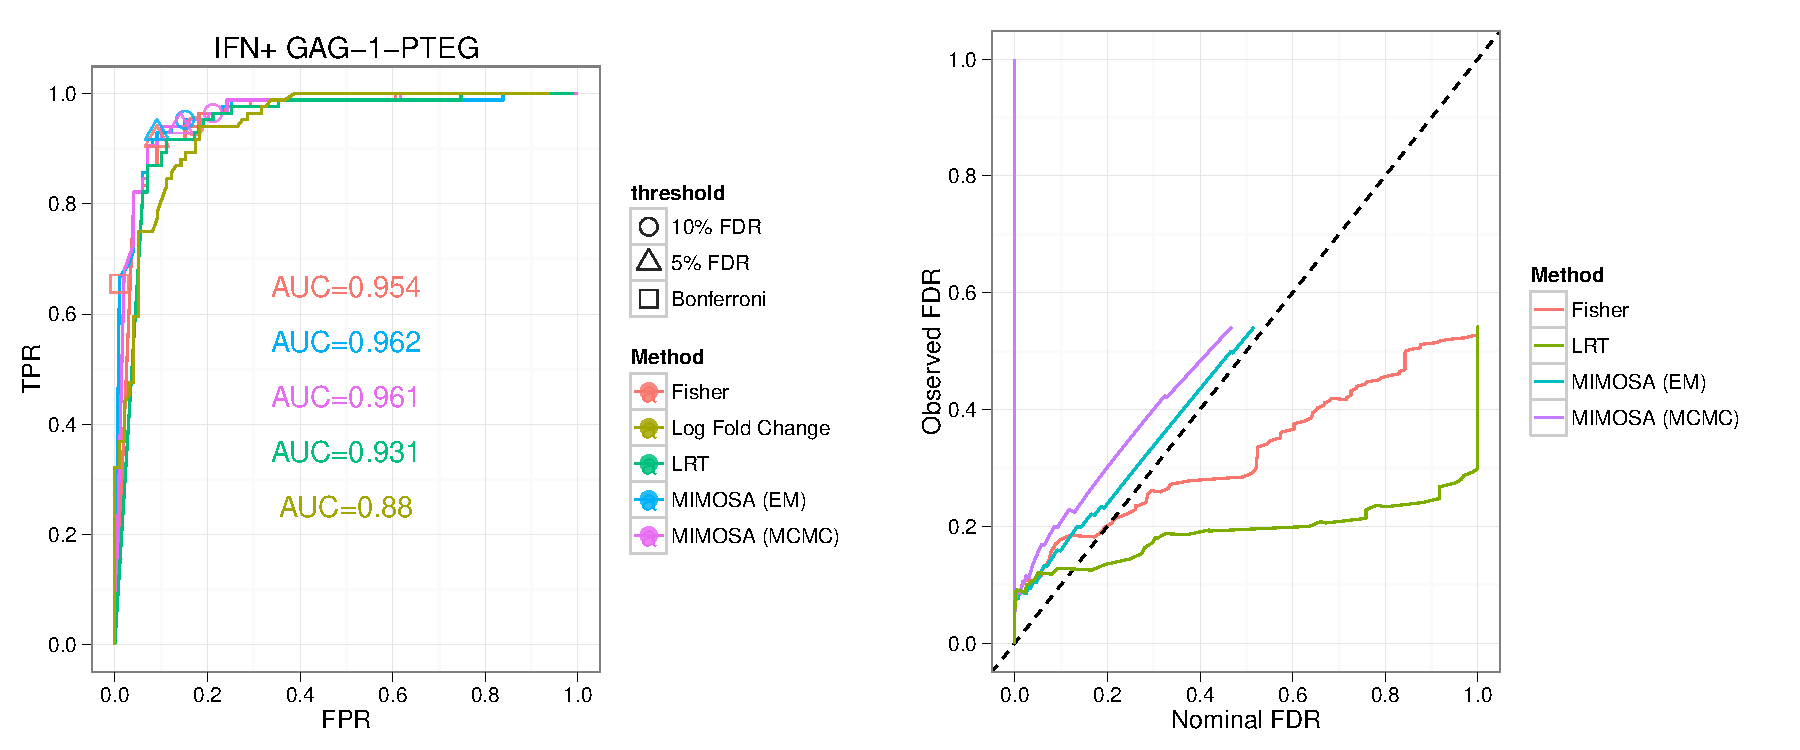
\includegraphics[width=.5\columnwidth]{Figures/9}};
    %\node[anchor=south west, inner sep=0] at (8,-11.25){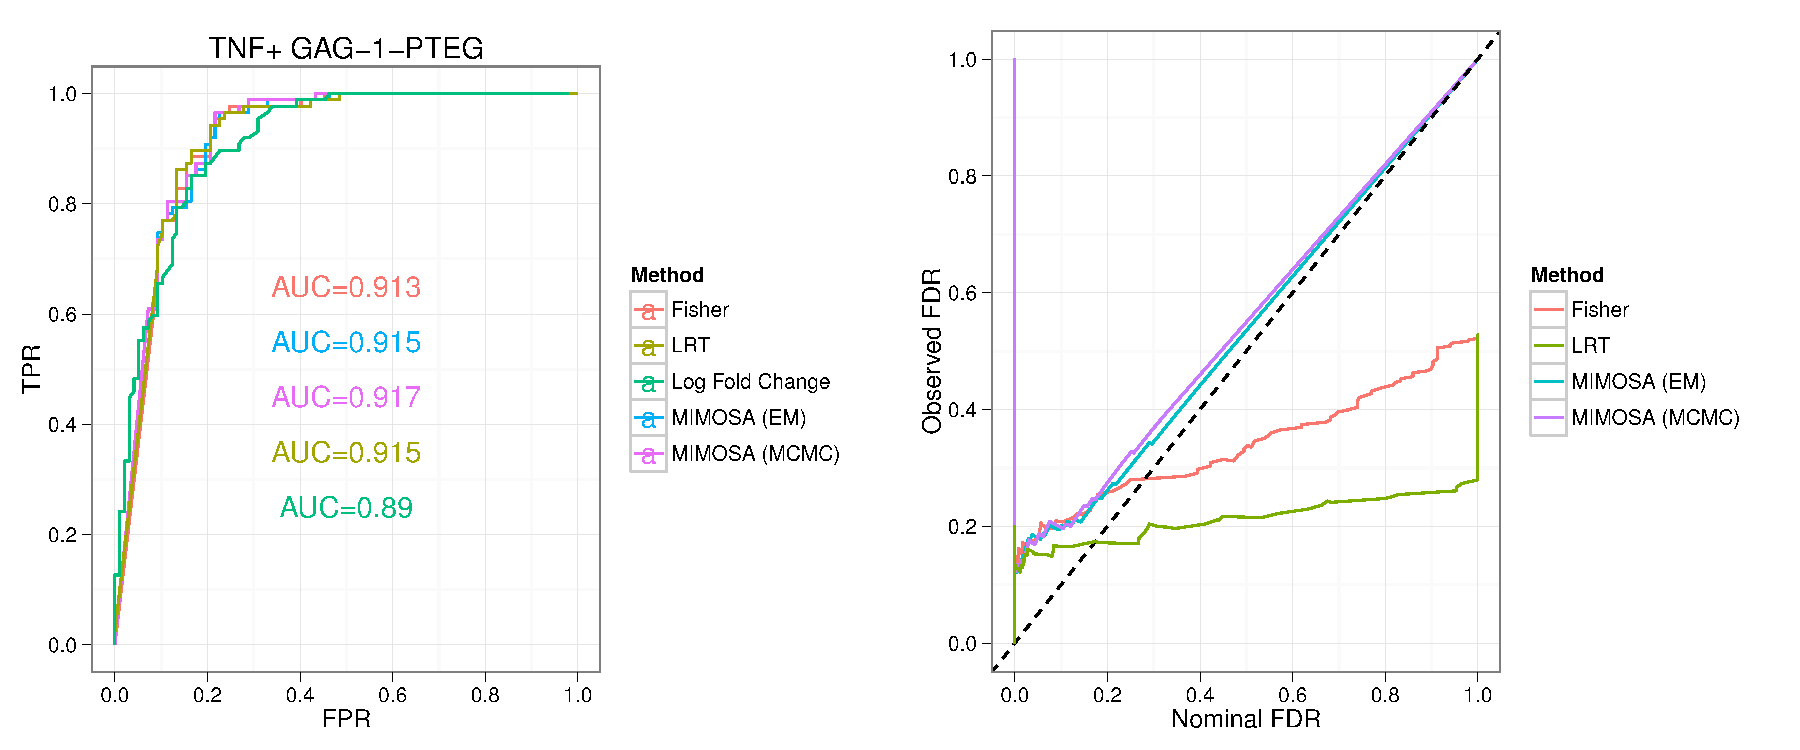
\includegraphics[width=.5\columnwidth]{Figures/10}};
    %\node[anchor=south west, inner sep=0] at (0,-15){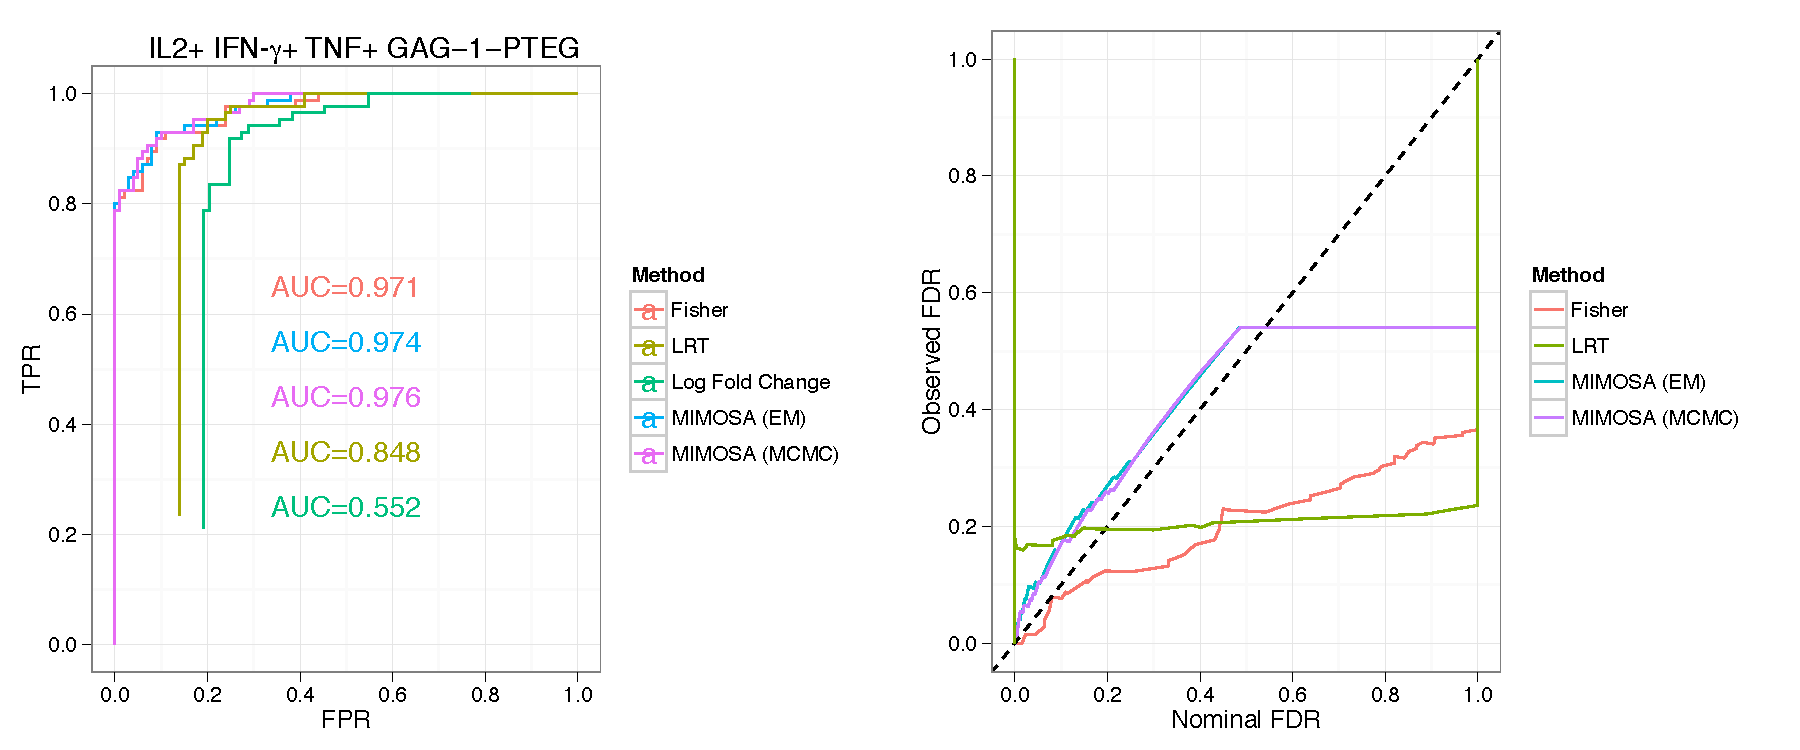
\includegraphics[width=.5\columnwidth]{Figures/11}};
    %\node[anchor=south west, inner sep=0] at (8,-15){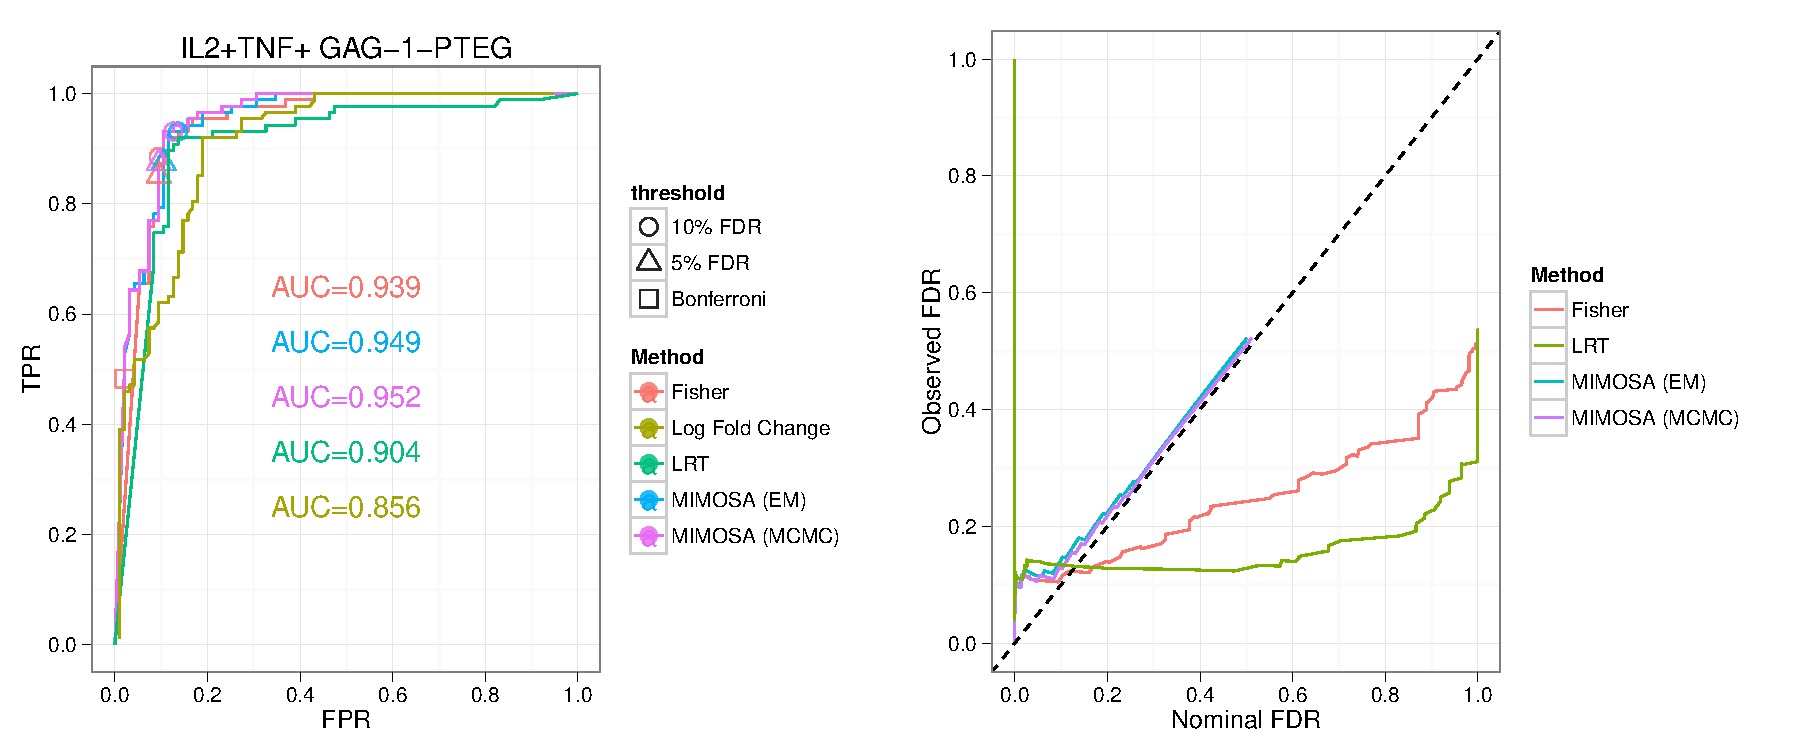
\includegraphics[width=.5\columnwidth]{Figures/13}};

  %  \node at (8,-4) [font=\small\sffamily] {F} ;
%    \node at (0,-7.75) [font=\small\sffamily] {G} ;
  %  \node at (8,-7.75) [font=\small\sffamily] {H} ;
   % \node at (0,-11.75) [font=\small\sffamily] {I} ;
   % \node at (8,-11.75) [font=\small\sffamily] {J} ;
    \end{tikzpicture}
   \caption{Comparison of MIMOSA on other cytokines and cytokine combinations for ENV-1-PTEG stimulated CD4+ T-cells from the HVTN065 trial.}
\label{webfig:HVTN065Results}
\end{figure}


\begin{figure} %  figure placement: here, top, bottom, or page
   \centering
\begin{tikzpicture} [auto,node distance=0cm]
    \node at (0,0) (A) {
    \begin{tikzpicture}
     \node[anchor=south west,inner sep=0] at (0,0) (c) {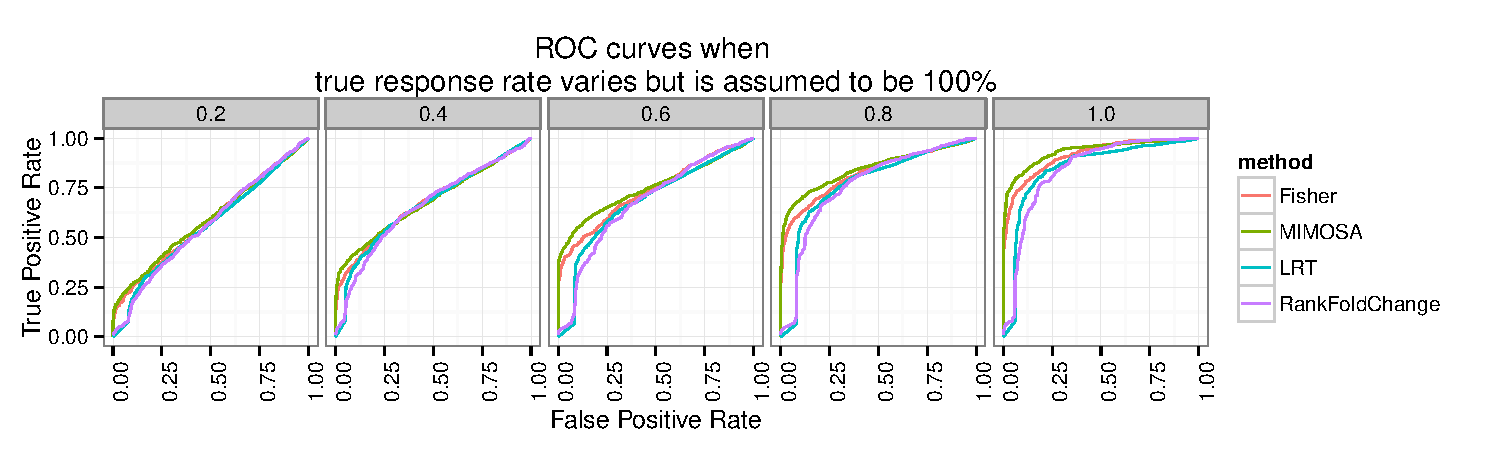
\includegraphics[width=0.75	\columnwidth]{Figures/competeROC.pdf}};
         \begin{scope} [x={(c.south east)},y={(c.north west)}]
                 \node at (0,1) [font=\tiny\sffamily] {A} ;
	\end{scope}
     \end{tikzpicture}
     };
     \node [below=of A] (B) {
     \begin{tikzpicture}
    \node[anchor=south west, inner sep=0] at (0,0) (d) {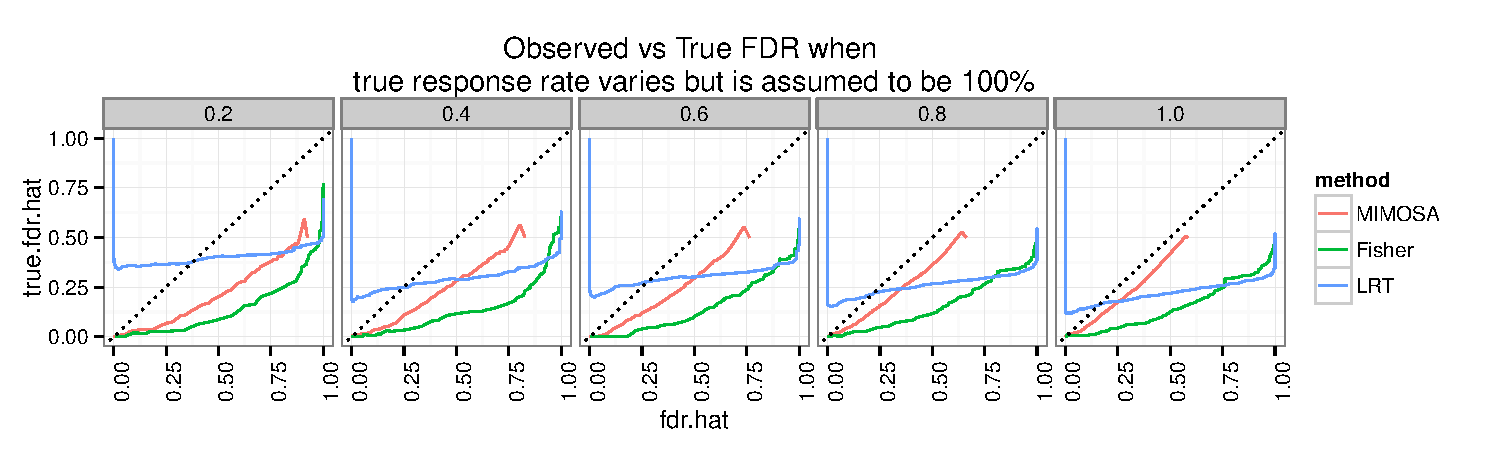
\includegraphics[width=0.75\columnwidth]{Figures/competeROCfdr.pdf}};
        \begin{scope} [x={(d.south east)},y={(d.north west)}]
            \node at (0,1) [font=\tiny\sffamily] {B} ;
\end{scope}
    \end{tikzpicture}
    };
  \end{tikzpicture}
   \caption{Effect of deviations of the assumptions of 100\% true responders at the post-vaccine time point on A) ROC and B) FDR curves. The true response rate is shown in the gray box above each plot.
}
   \label{webfig:simulations_competeroc}
\end{figure}
%\begin{figure}[htbp] %  figure placement: here, top, bottom, or page
%   \centering
%%   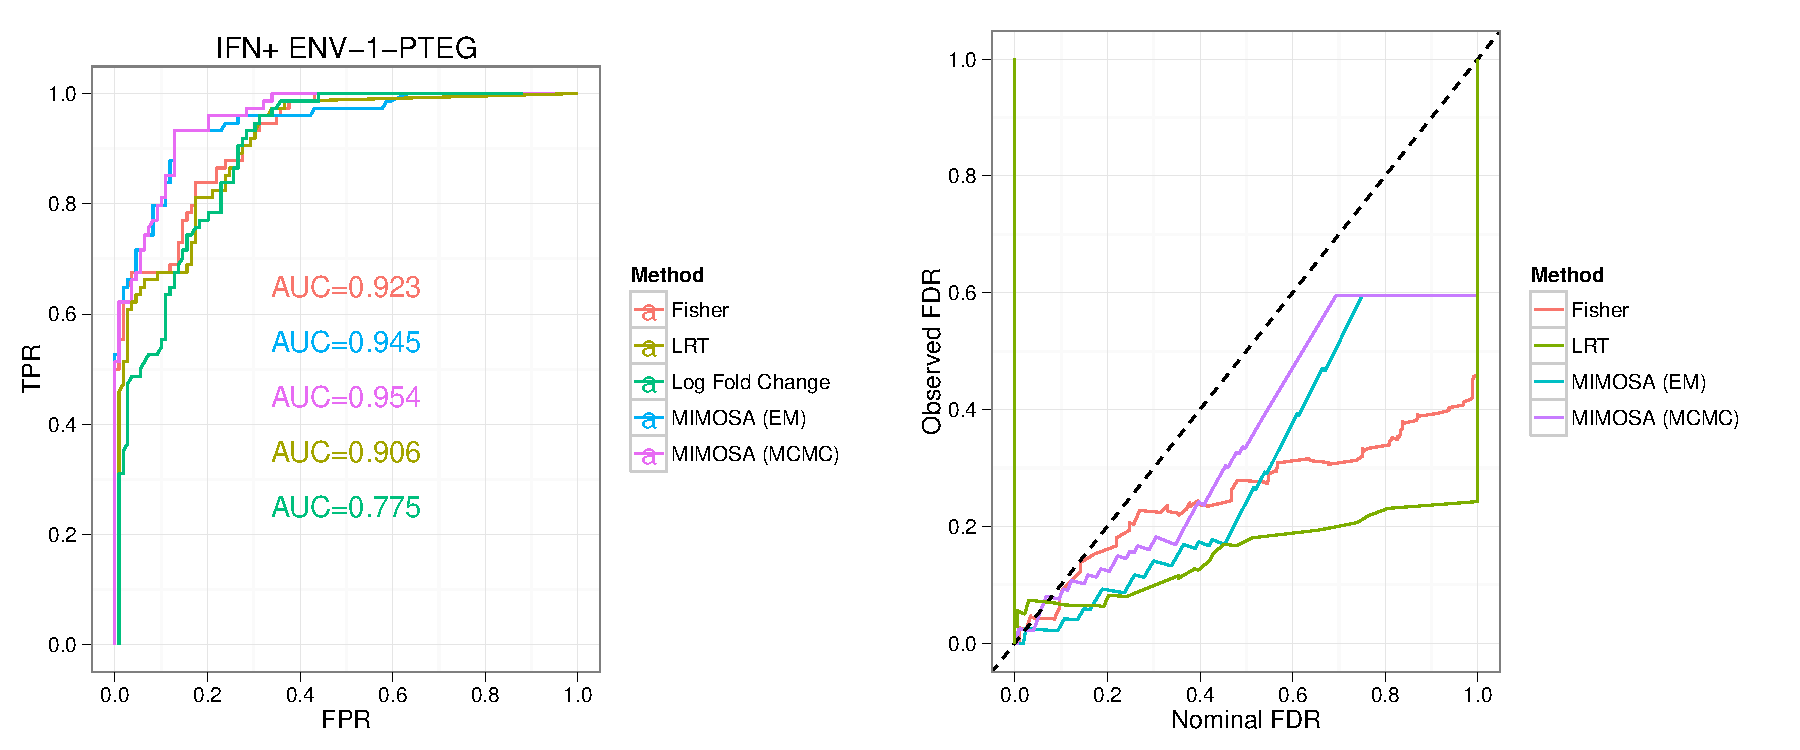
\includegraphics[width=.75\columnwidth]{Figures/2}\\
%%   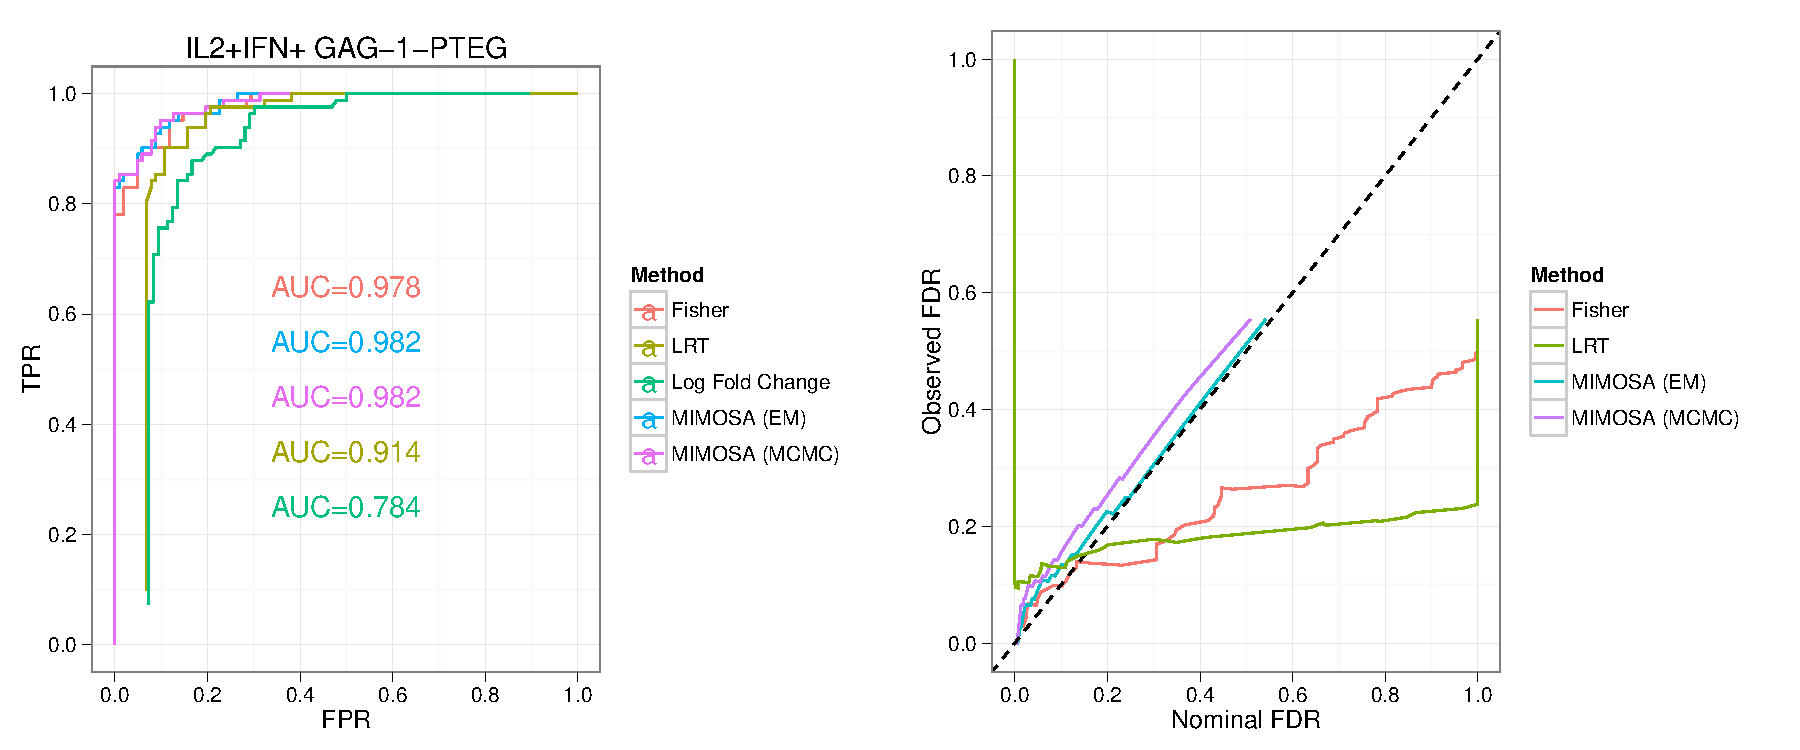
\includegraphics[width=.75\columnwidth]{Figures/12}
%\begin{tikzpicture}
%    \node[anchor=south west, inner sep=0] at (0,0){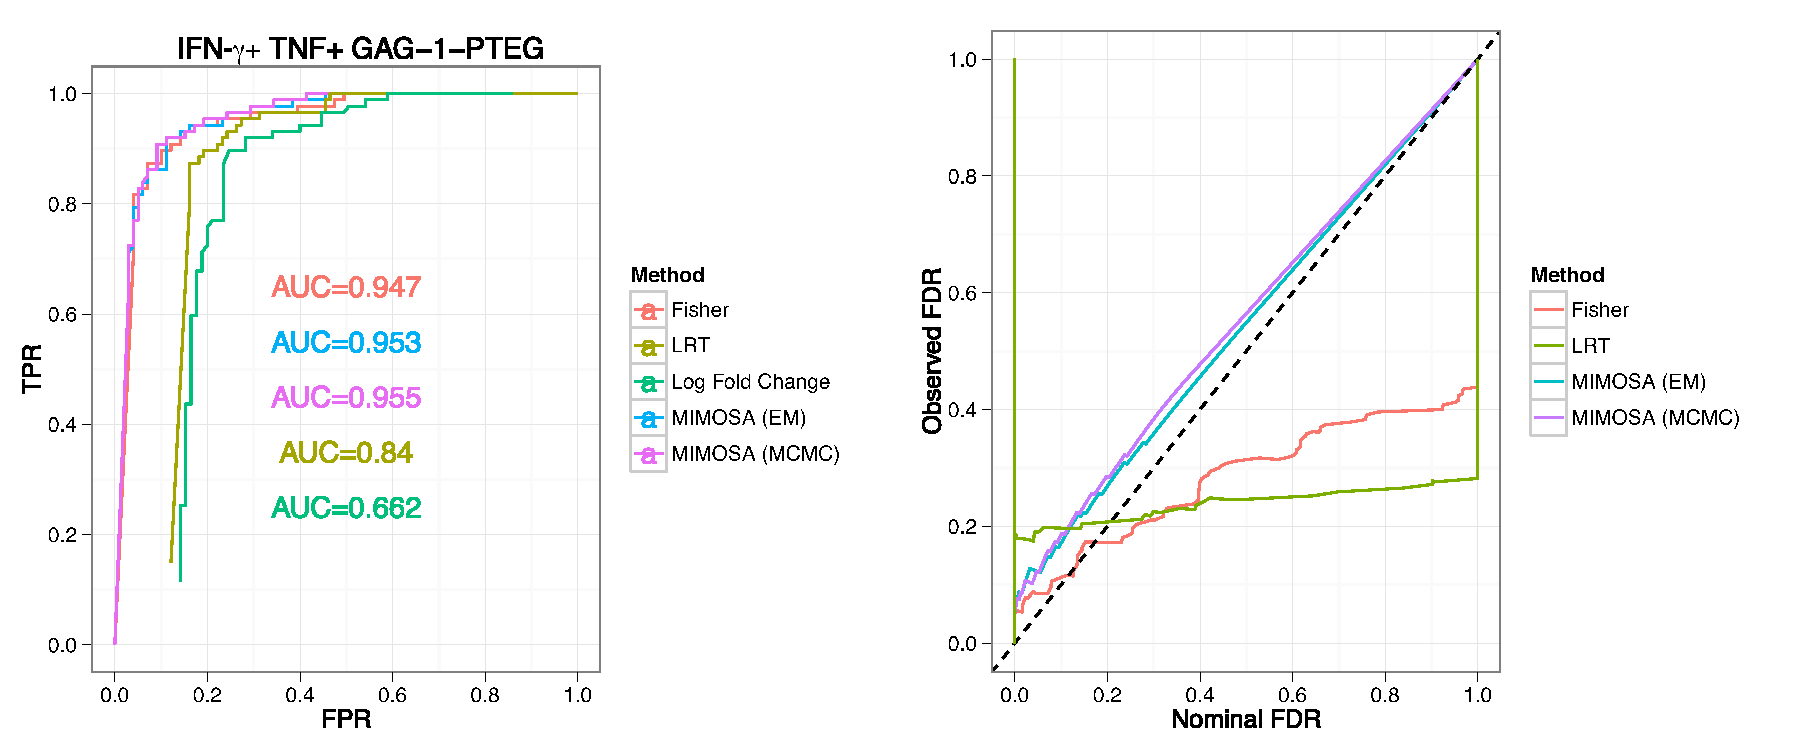
\includegraphics[width=.5\columnwidth]{Figures/14}};
%    \node[anchor=south west, inner sep=0] at (8,0){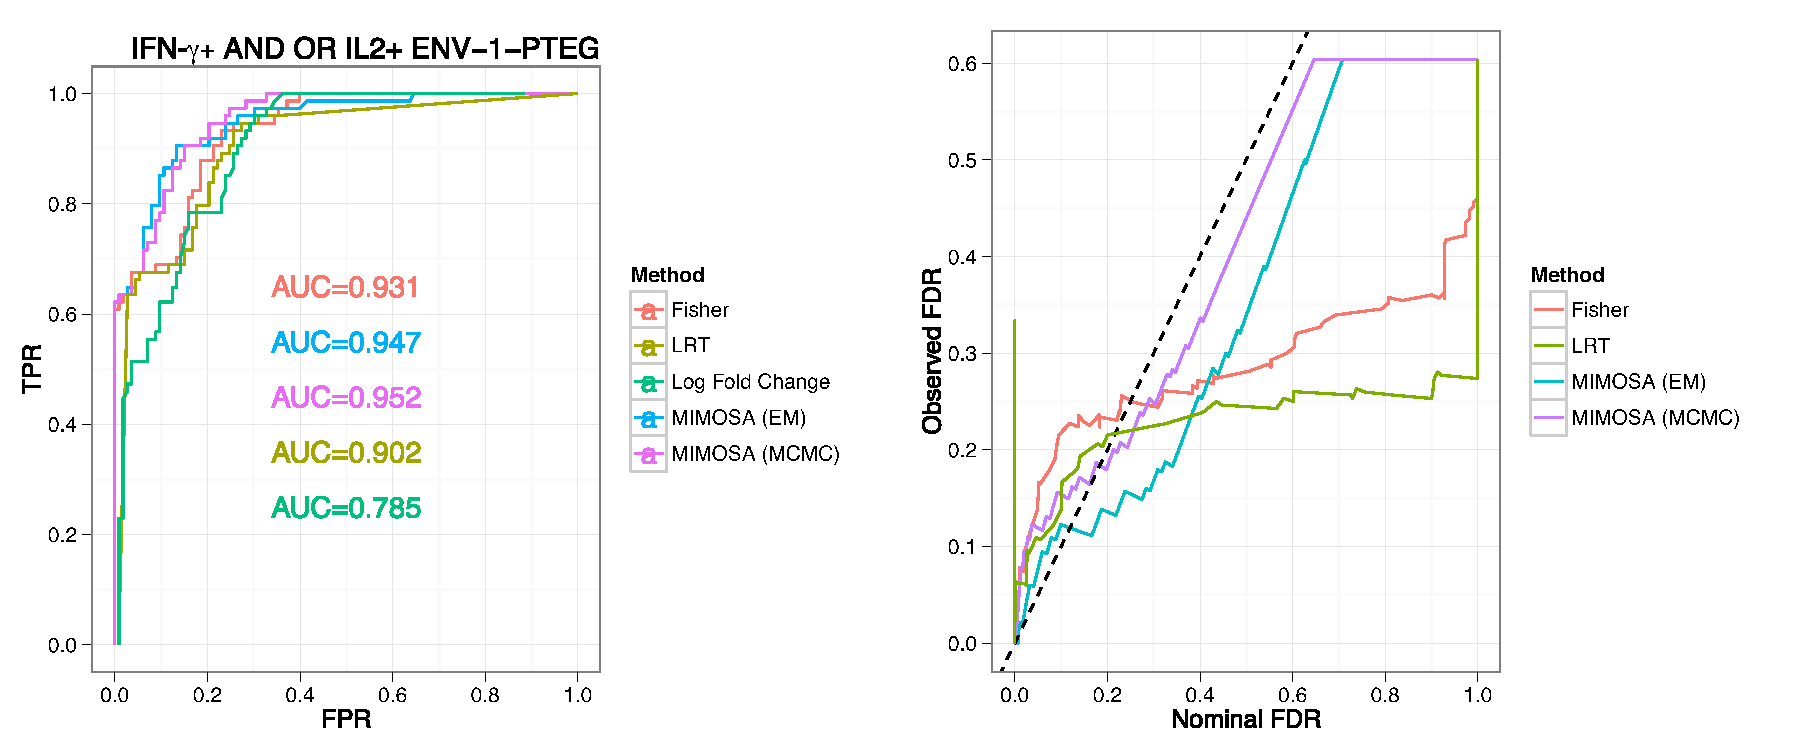
\includegraphics[width=.5\columnwidth]{Figures/15}};
%    \node[anchor=south west, inner sep=0] at (0,-3.75){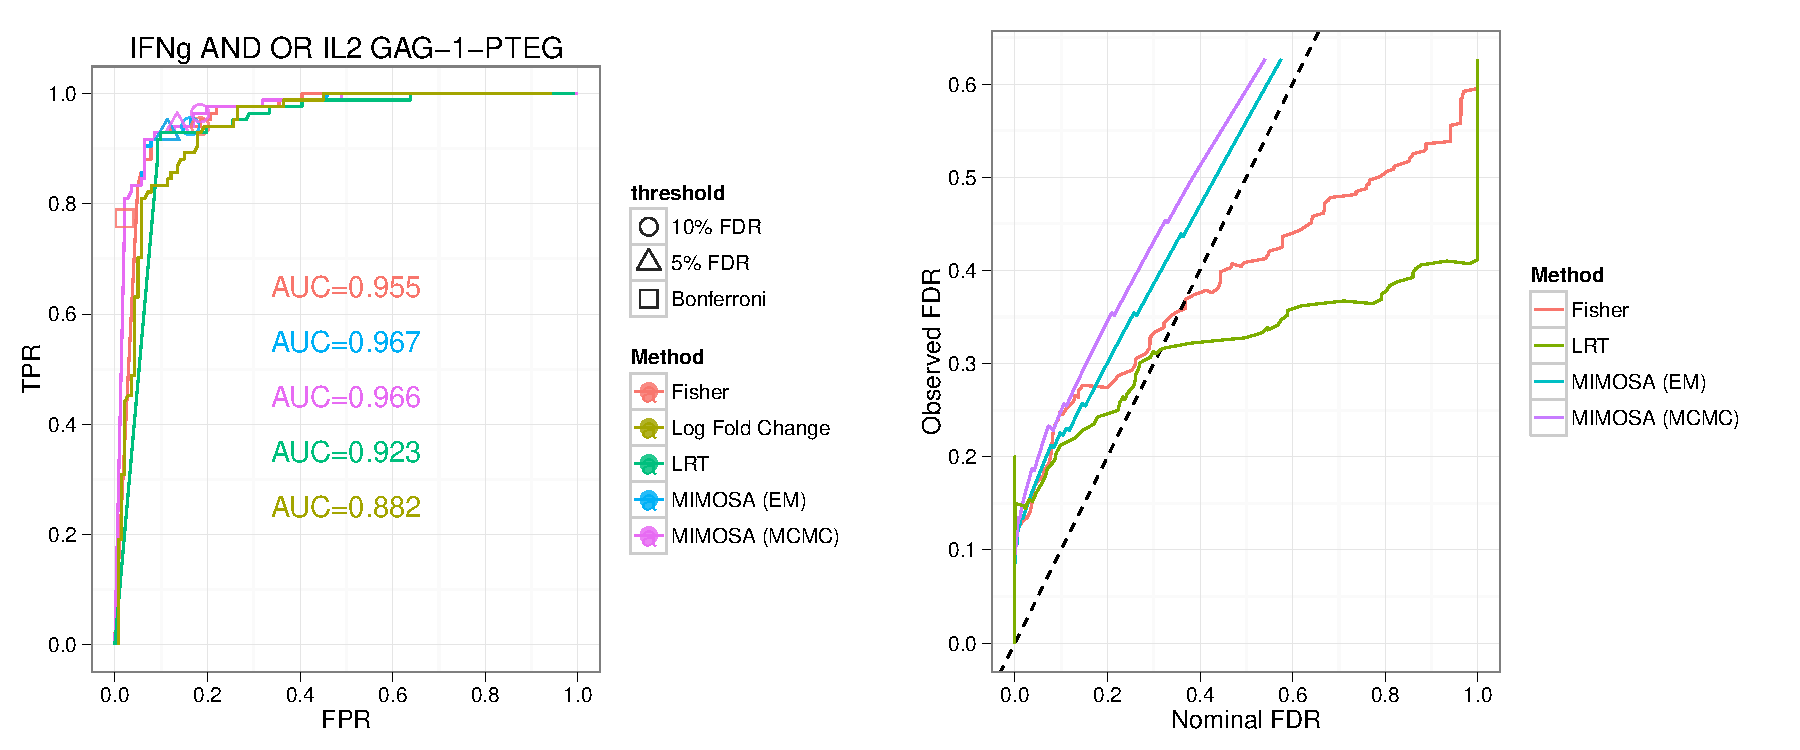
\includegraphics[width=.5\columnwidth]{Figures/16}};
%
%
%    \node at (0,3.4) [font=\small\sffamily] {A} ;
%    \node at (8,3.4) [font=\small\sffamily] {B} ;
%    \node at (0,-0.5) [font=\small\sffamily] {C} ;
%    \end{tikzpicture}
%   \caption{Comparison of MIMOSA on other cytokines and cytokine combinations for ENV-1-PTEG and GAG-1-PTEG stimulated CD4+ T-cells from the HVTN065 trial.}
%\label{fig:HVTN065ResultsCont}
%\end{figure}

 \begin{figure}
   \centering
   \begin{tikzpicture} [auto,node distance=0cm]
     \node at (0,0) (A) {
       \begin{tikzpicture}
         \node[anchor=south west,inner sep=0] at (0,0) (c) {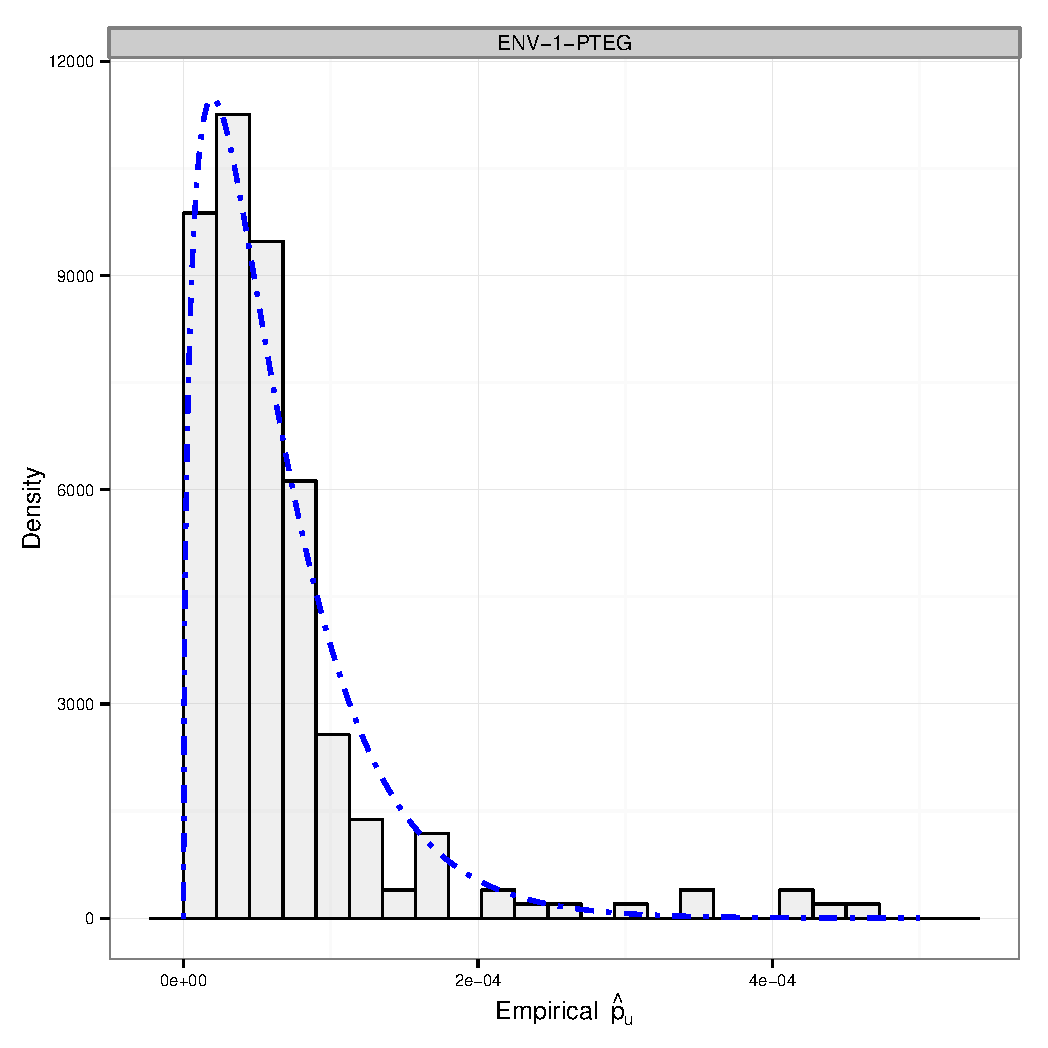
\includegraphics[width=0.4\columnwidth]{Figures/post_density_plots.pdf}};
         \begin{scope} [x={(c.south east)},y={(c.north west)}]
           \node at (0,1) [font=\tiny\sffamily] {A} ;
         \end{scope}
       \end{tikzpicture}
      };
    \end{tikzpicture}
    \caption{Histogram of the empirical proportions of unstimulated cells
      and overlaid posterior densities of the beta distribution with
      $\alpha^{(u)}$ and $\beta^{(u)}$ estimated from the data for ENV-1-PTEG
      stimulated, IFN--$\gamma$+, CD4+ T--cells, demonstrating that the assumption of a common distribution for $p_{iu}$ across subjects is reasonable. }
   \label{fig:empiricalpdist}
 \end{figure}



\begin{figure} %  figure placement: here, top, bottom, or page
   \centering
\begin{tikzpicture} [auto,node distance=0cm]
    \node at (0,0) (A) {
    \begin{tikzpicture}
     \node[anchor=south west,inner sep=0] at (0,0) (c) {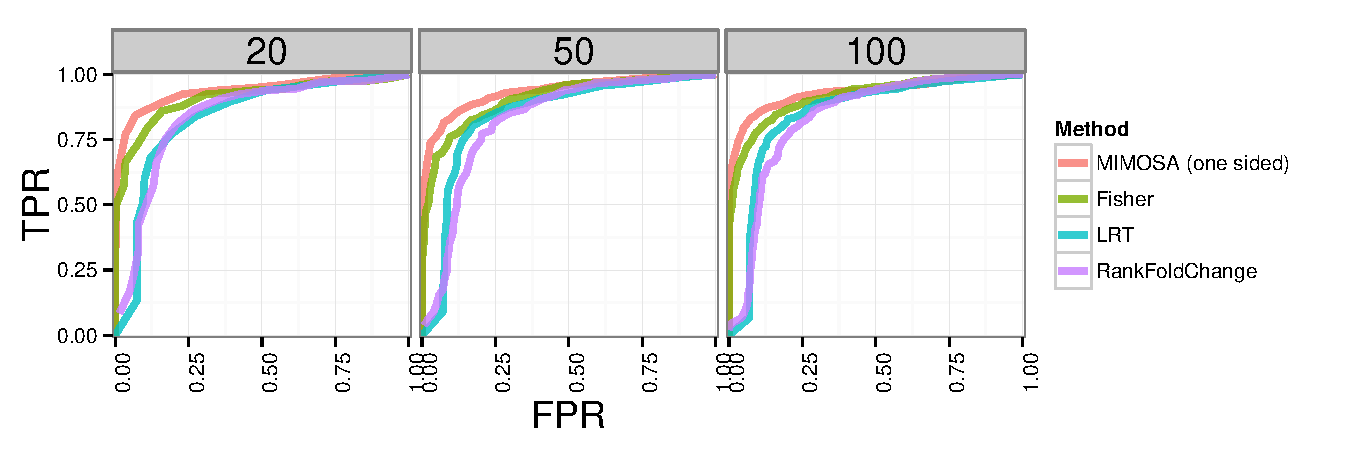
\includegraphics[width=0.75	\columnwidth]{Figures/Sim_OneSided_ROC_varyNobs.pdf}};
         \begin{scope} [x={(c.south east)},y={(c.north west)}]
                 \node at (0,1) [font=\tiny\sffamily] {A} ;
	\end{scope}
     \end{tikzpicture}
     };
     \node [below=of A] (B) {
     \begin{tikzpicture}
    \node[anchor=south west, inner sep=0] at (0,0) (d) {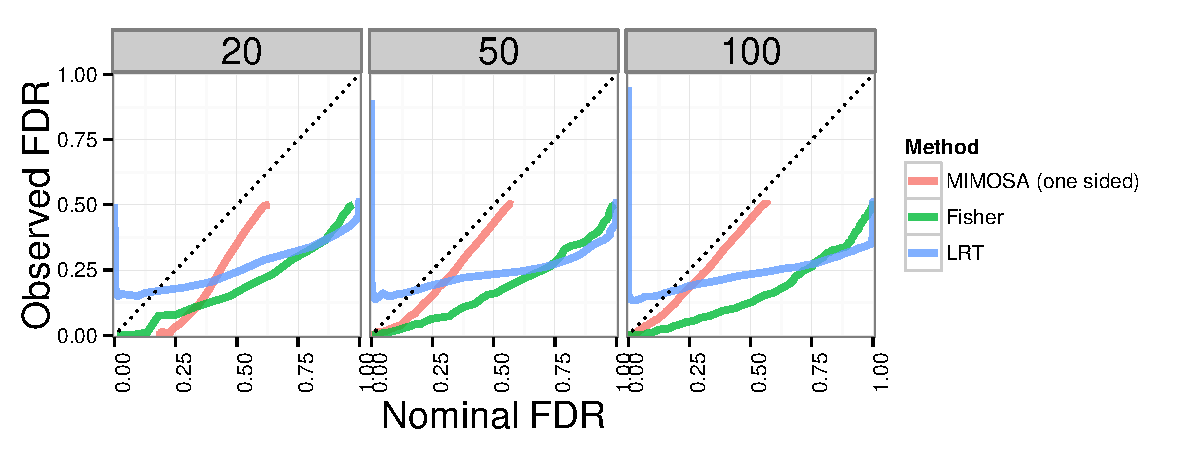
\includegraphics[width=0.75\columnwidth]{Figures/Sim_OneSided_FDR_varyNobs.pdf}};
        \begin{scope} [x={(d.south east)},y={(d.north west)}]
            \node at (0,1) [font=\tiny\sffamily] {B} ;
\end{scope}
    \end{tikzpicture}
    };
  \end{tikzpicture}
   \caption{One--sided MIMOSA model fit to simulated data with 50K cells and varying values of I (number of observations). A) Average ROC curves from 10 simulations for 20, 50 and 100 observations. B) Average observed and nominal FDR from 10 simulations for 20, 50, and 100 observations. }
   \label{webfig:simulations_Nobs}
\end{figure}
\clearpage


\begin{figure} %  figure placement: here, top, bottom, or page
   \centering
\begin{tikzpicture} [auto,node distance=0cm]
%\node at (0,0) (A) {
%\begin{tikzpicture}
%    \node[anchor=south west,inner sep=0] at (0,0) (a) {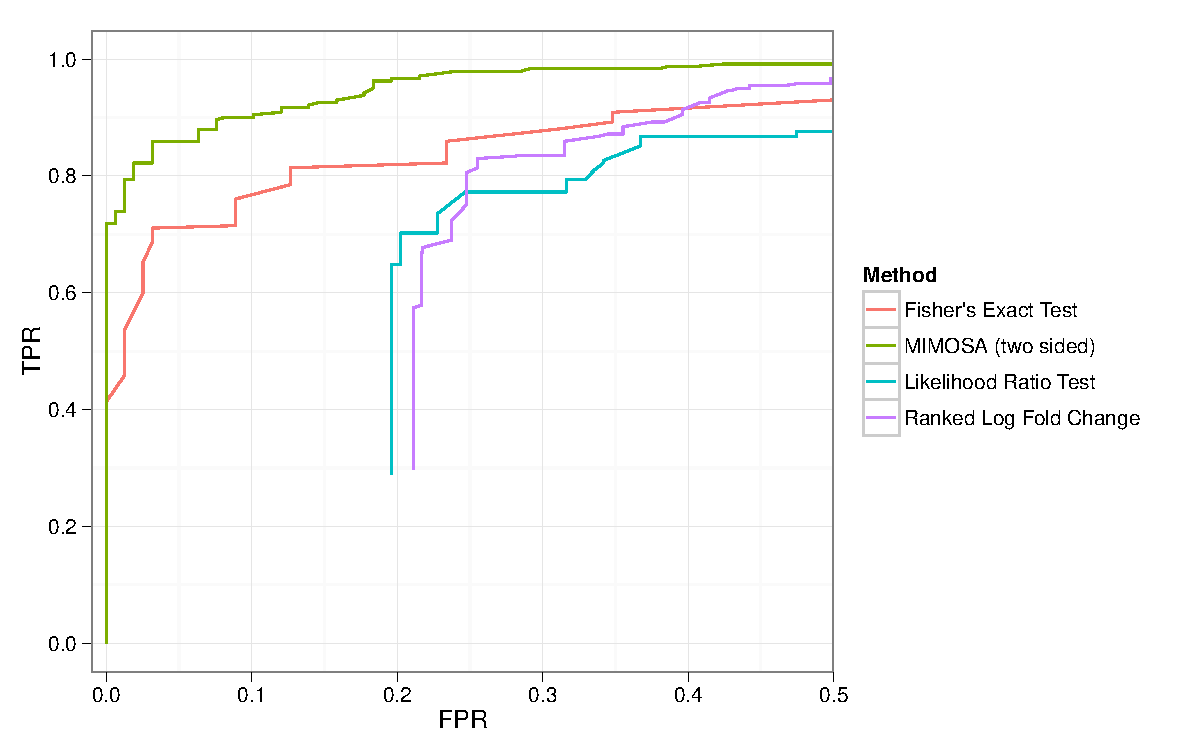
\includegraphics[width=0.4\columnwidth]{Figures/Sim_Twosided_ROC_5000.pdf}};
%    \begin{scope} [x={(a.south east)},y={(a.north west)}]
%        \node at (0,1) [font=\small\sffamily] {A} ;
%    \end{scope}
%    \end{tikzpicture}
%    };
%    \node [right=of A] (B) {
%    \begin{tikzpicture}
%    \node[anchor=south west, inner sep=0] at (0,0) (b) {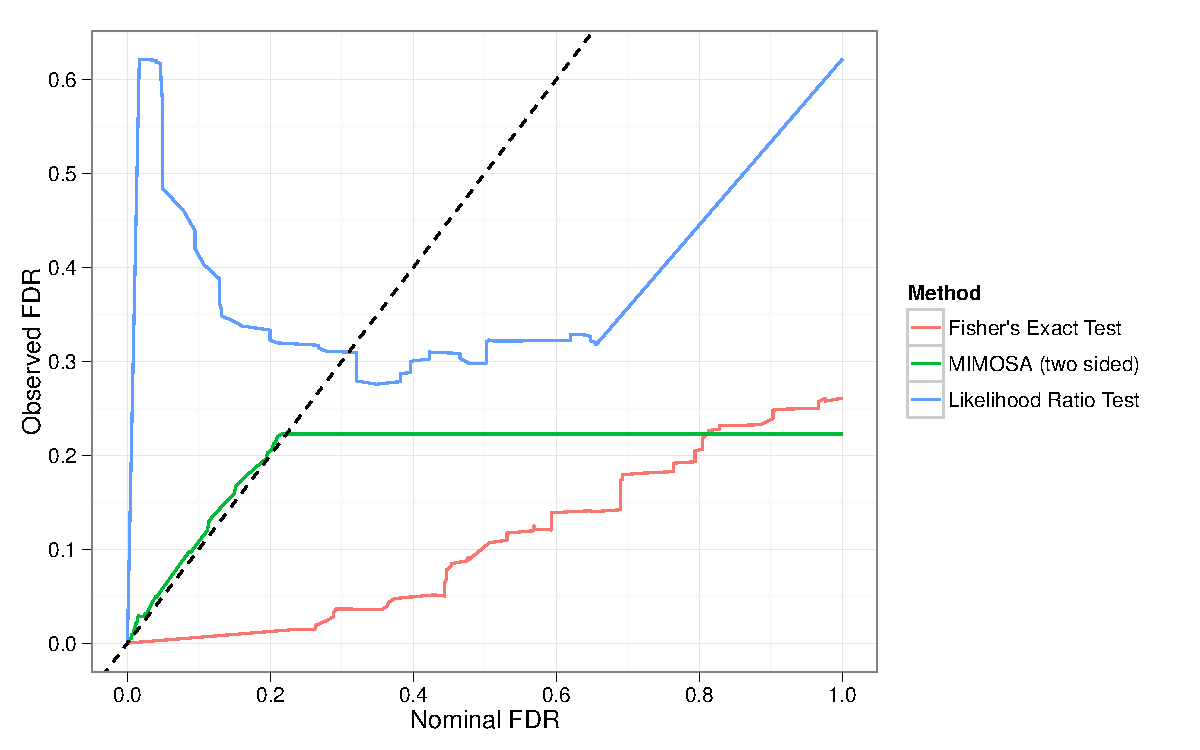
\includegraphics[width=0.4\columnwidth]{Figures/Sim_Twosided_FDR_5000.pdf}};
%        \begin{scope} [x={(b.south east)},y={(b.north west)}]
%        \node at (0,1) [font=\small\sffamily] {B} ;
%        \end{scope}
%    \end{tikzpicture}
%    };
    \node at (0,0) (A) {
    \begin{tikzpicture}
     \node[anchor=south west,inner sep=0] at (0,0) (c) {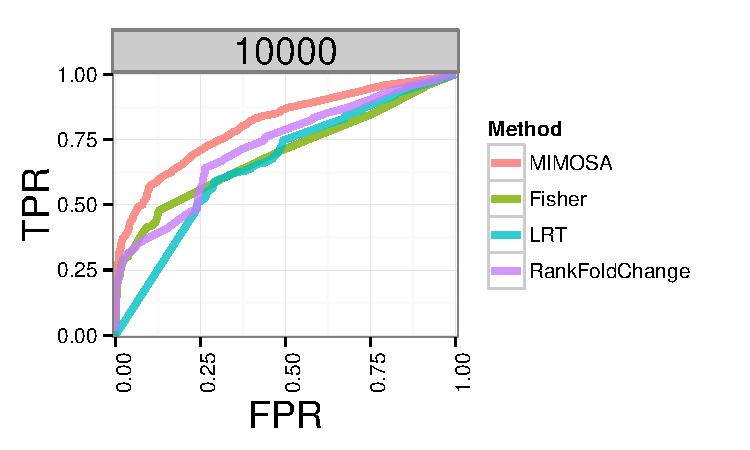
\includegraphics[width=0.4\columnwidth]{Figures/Sim_Truncated_ROC_10K.pdf}};
         \begin{scope} [x={(c.south east)},y={(c.north west)}]
                 \node at (0,1) [font=\tiny\sffamily] {A} ;
	\end{scope}
     \end{tikzpicture}
     };
     \node [right=of A] (B) {
     \begin{tikzpicture}
    \node[anchor=south west, inner sep=0] at (0,0) (d) {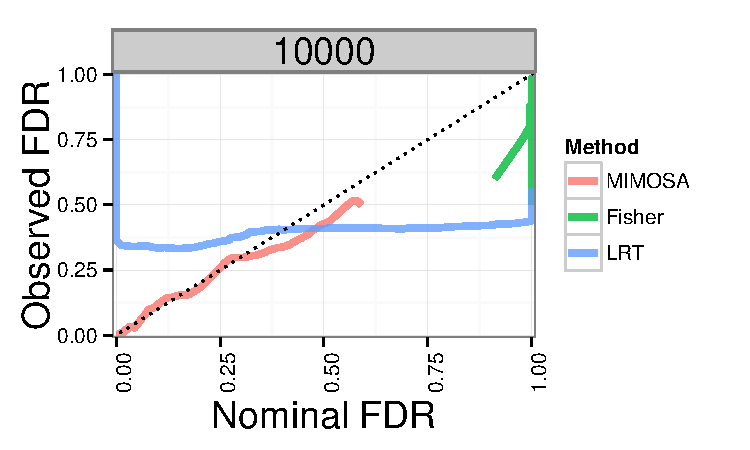
\includegraphics[width=0.4\columnwidth]{Figures/Sim_Truncated_FDR_10K.pdf}};
        \begin{scope} [x={(d.south east)},y={(d.north west)}]
            \node at (0,1) [font=\tiny\sffamily] {B} ;
\end{scope}
    \end{tikzpicture}
    };
  \node [below=of A] (C) {
\begin{tikzpicture}
    \node[anchor=south west,inner sep=0] at (0,0) (e) {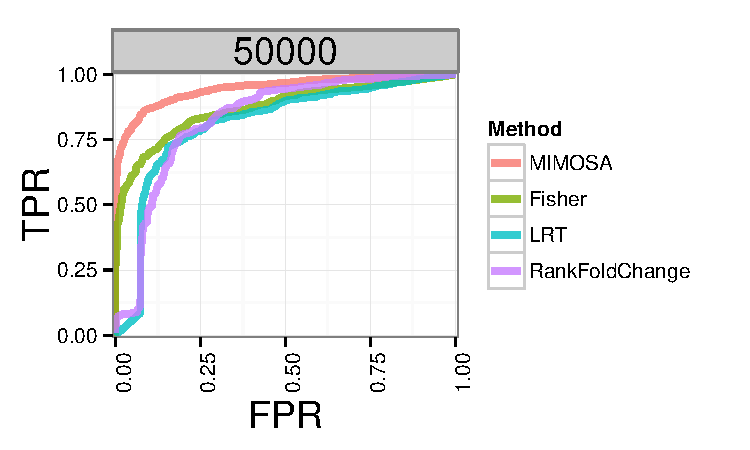
\includegraphics[width=0.4\columnwidth]{Figures/Sim_Truncated_ROC_50K.pdf}};
    \begin{scope} [x={(e.south east)},y={(e.north west)}]
        \node at (0,1) [font=\tiny\sffamily] {C} ;
    \end{scope}
    \end{tikzpicture}
    };
    \node [right=of C] (D) {
    \begin{tikzpicture}
    \node[anchor=south west, inner sep=0] at (0,0) (f) {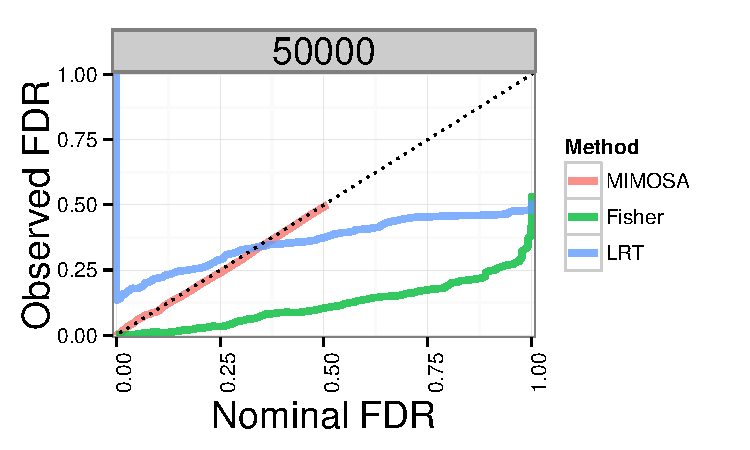
\includegraphics[width=0.4\columnwidth]{Figures/Sim_Truncated_FDR_50K.pdf}};
        \begin{scope} [x={(f.south east)},y={(f.north west)}]
        \node at (0,1) [font=\tiny\sffamily] {D} ;
        \end{scope}
    \end{tikzpicture}
    };
%     \node [below=of C] (E) {
%     \begin{tikzpicture}
%      \node[anchor=south west,inner sep=0] at (0,0) (g) {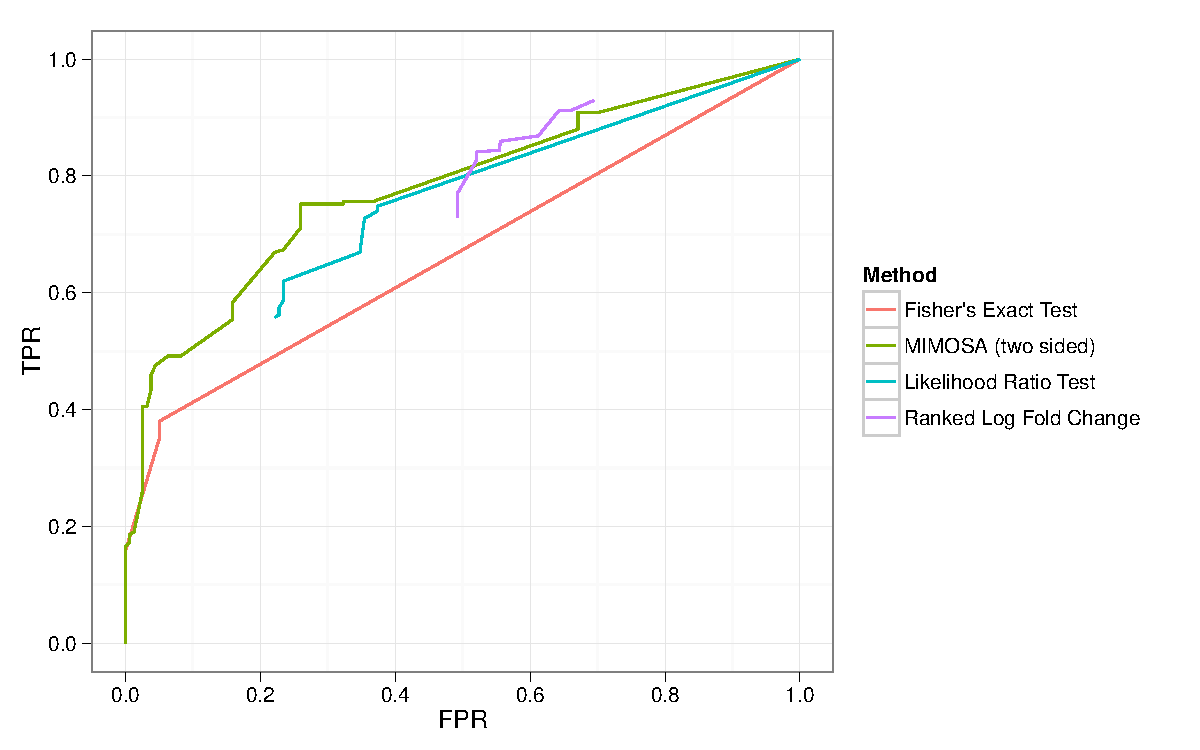
\includegraphics[width=0.4\columnwidth]{Figures/Sim_Twosided_ROC_1000.pdf}};
%          \begin{scope} [x={(g.south east)},y={(g.north west)}]
%                  \node at (0,1) [font=\tiny\sffamily] {E} ;
% 	\end{scope}
%      \end{tikzpicture}
%      };
%      \node [right=of E] (F) {
%      \begin{tikzpicture}
%     \node[anchor=south west, inner sep=0] at (0,0) (h) {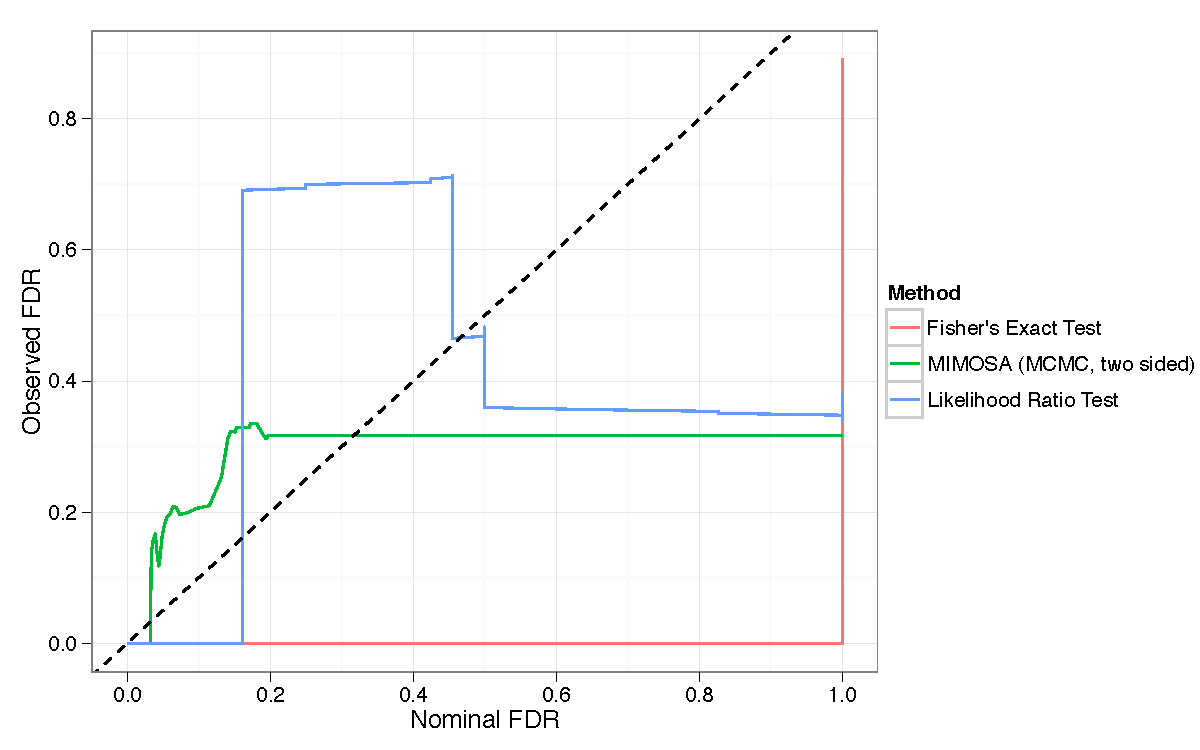
\includegraphics[width=0.4\columnwidth]{Figures/Sim_Twosided_FDR_1000.pdf}};
%         \begin{scope} [x={(h.south east)},y={(h.north west)}]
%             \node at (0,1) [font=\tiny\sffamily] {F} ;
% \end{scope}
%     \end{tikzpicture}
%     };
 \end{tikzpicture}
   \caption{Unconstrained MIMOSA model fit to two-sided data with small
     counts  and to  data from a model
     violating model assumptions.  For two-sided data A) the average ROC from 10 simulation
     with N=10,000 cells. B) the average observed and nominal FDR from
     10 simulations with N=10,000 cells. Data was simulated from a model where proportions were
     sampled from a truncated normal distribution over $[0,1]$ rather
     than a Beta distribution. C) Average ROC for N=50,000
     cells D) Average observed and nominal FDR for N=50,000 cells.
}
   \label{webfig:simulations_trunc}
\end{figure}
\clearpage

\begin{figure} %  figure placement: here, top, bottom, or page
   \centering
   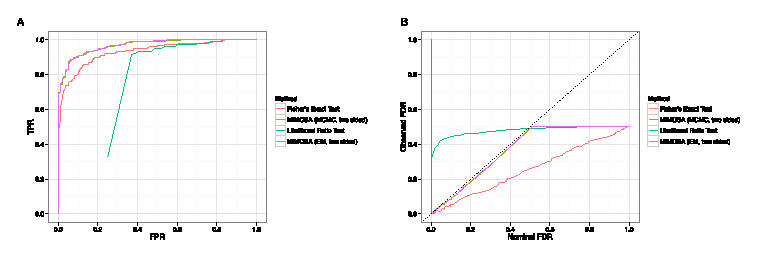
\includegraphics{TIKZFig5.eps}
%\begin{tikzpicture} [auto, node distance=0cm]
%\node at (0,0) (A) {
%\begin{tikzpicture}
%    \node[anchor=south west, inner sep=0] at (0,0) (foo) {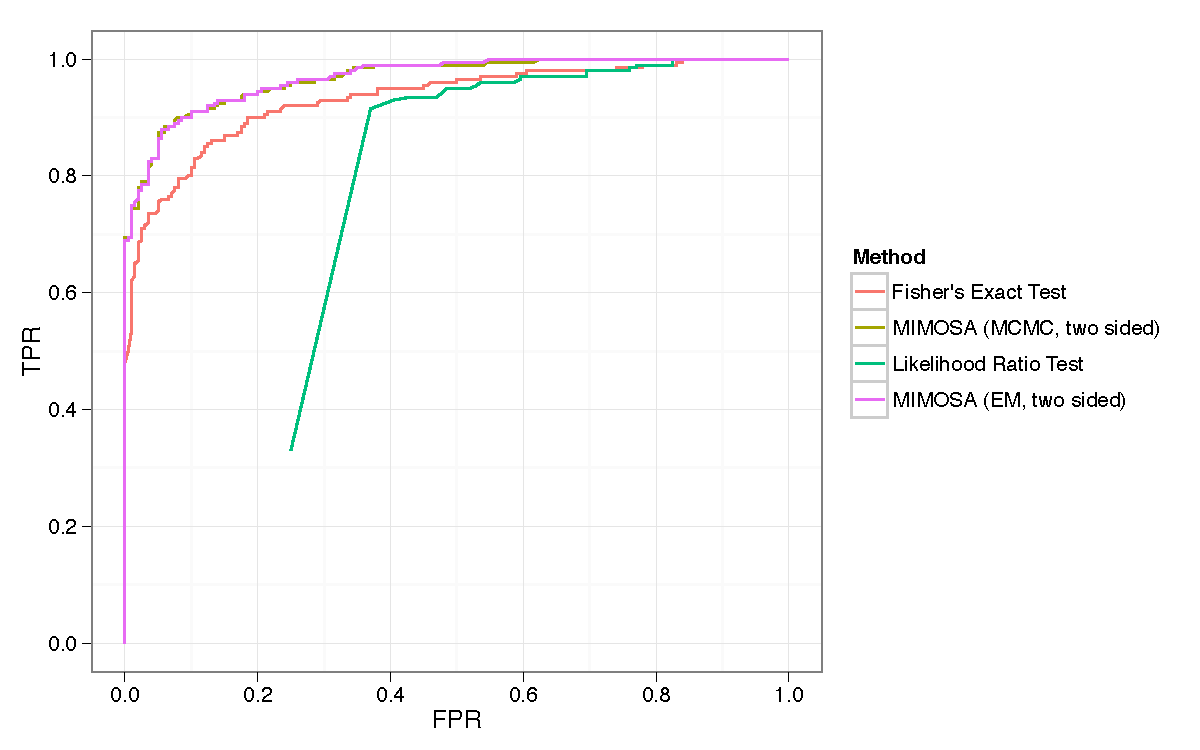
\includegraphics[width=0.47\columnwidth]{Figures/Multivariate_Sims_ROC_rev.pdf}};
%\begin{scope} [x={(foo.south east)},y={(foo.north west)}]
%    \node at (0,1) [font=\small\sffamily] {A} ;
%\end{scope}
%\end{tikzpicture}
%};
%\node [right=of A] (B) {
%\begin{tikzpicture}
%   \node[anchor=south west, inner sep=0] at (0,0) (bar) {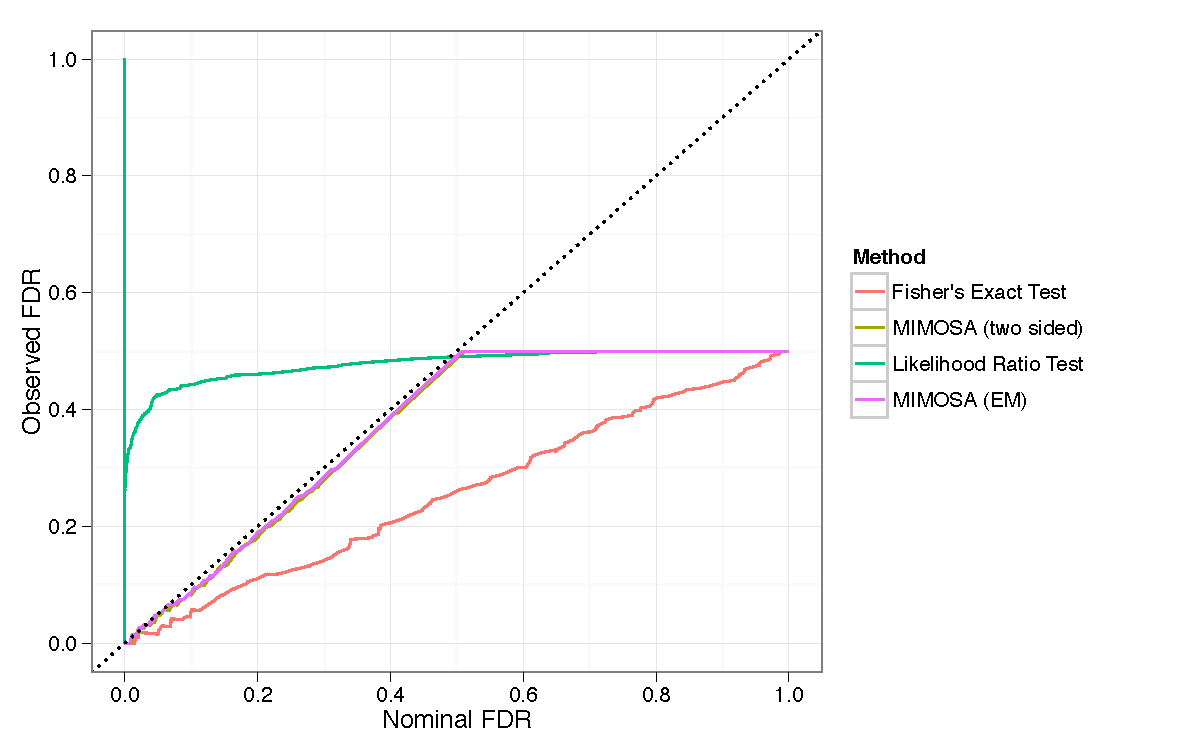
\includegraphics[width=0.47\columnwidth]{Figures/Multivariate_Sims_FDR_rev.pdf}};
%   \begin{scope} [x={(bar.south east)},y={(bar.north west)}]
%       \node at (0,1) [font=\small\sffamily] {B} ;
%\end{scope}
%\end{tikzpicture}
%};
%\end{tikzpicture}
   \caption{Multivariate simulations from a two-sided model. Ten, eight-dimensional data sets were simulated from a two-sided model with an effect sizes of $2.5\times 10^{-3}$ and $-2.5\times 10^{-3}$ in two of the eight dimensions (N=1,500). Multivariate MIMOSA was compared against Fisher's exact test, and the likelihood ratio test. A) Average ROC curves for the competing methods over 10 simulations. B) Average observed and nominal false discovery rate for each method over 10 simulations. This figure appears in color in the electronic version of this article.}
   \label{fig:mvsimulations}
\end{figure}


\begin{figure} %  figure placement: here, top, bottom, or page
   \centering
\begin{tikzpicture} [auto,node distance=0cm]
    \node at (0,0) (A) {
    \begin{tikzpicture}
     \node[anchor=south west,inner sep=0] at (0,0) (c) {\includegraphics[width=0.75	\columnwidth]{Figures/volcanoplots.pdf}};
         \begin{scope} [x={(c.south east)},y={(c.north west)}]
                 \node at (0,1) [font=\tiny\sffamily] {A} ;
	\end{scope}
     \end{tikzpicture}
     };
    \end{tikzpicture}
   \caption{Volcano plots of effect size vs posterior probability of response for each model fit to each cytokine in the ICS data set. Green points indicate subjects called responders for that cytokine and stimulation at a 1\% FDR threshold (adjusted across subjects within cytokine subset). Red points indicate non-responders.
}
   \label{webfig:simulations_Nobs}
\end{figure}
\clearpage

\bibliographystyle{biorefs}
\bibliography{MIMOSA}


\end{document}
